\section{Evaluation}
\label{sec:result}
% use one net to represent a complicated scene
% we still have other option for real-time, like streaming
\note{
Ablation studies for the network training/losses
Target scene | Foveated target scene | NeRF | network predicted images ---> at least 4 different scenes.
streaming time for 4-5 different scenes: full resolution vs our network prediction for “same data size”
image quality of rendered scene vs our network prediction for “same amount of streaming time”
User study results
Table on performance comparison, streaming time, PSNR, SSIM, etc
}%note
With a variety of scenes as shown in \Cref{fig:results:comparison2}, we evaluate our method with subjective studies (\Cref{sec:study:user}), objective analysis (\Cref{sec:study:quality}), and intra-system efficiency (\Cref{sec:study:intra}).
\begin{figure*}[htb]
    \centering
    \begin{minipage}{0.32\linewidth} %full res
        \subfloat[gas scene(\textbf{GT})]{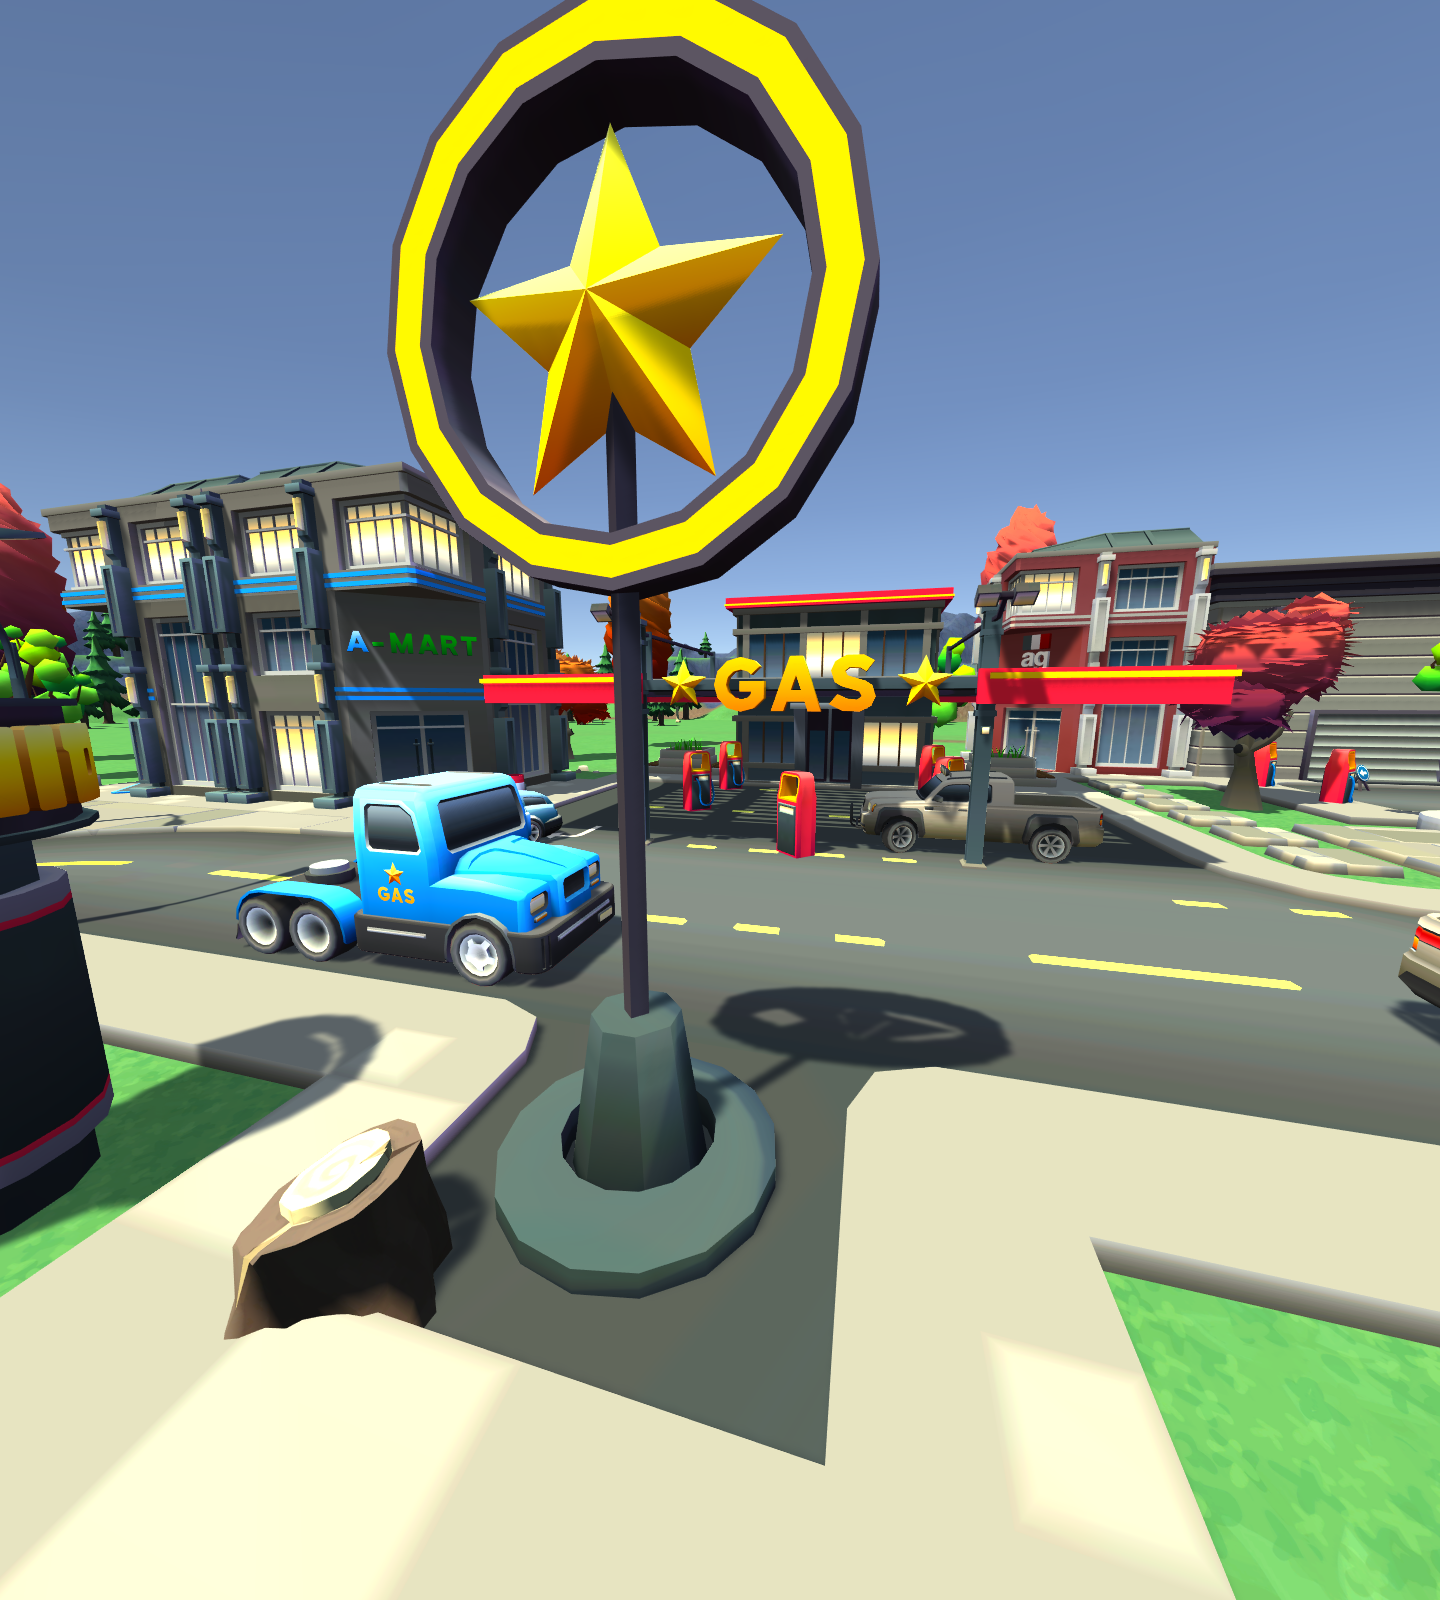
\includegraphics[width=0.96\linewidth]{TOG/figs/gas_gt4.png}}
        
        \subfloat[minecraft scene(\textbf{GT})]{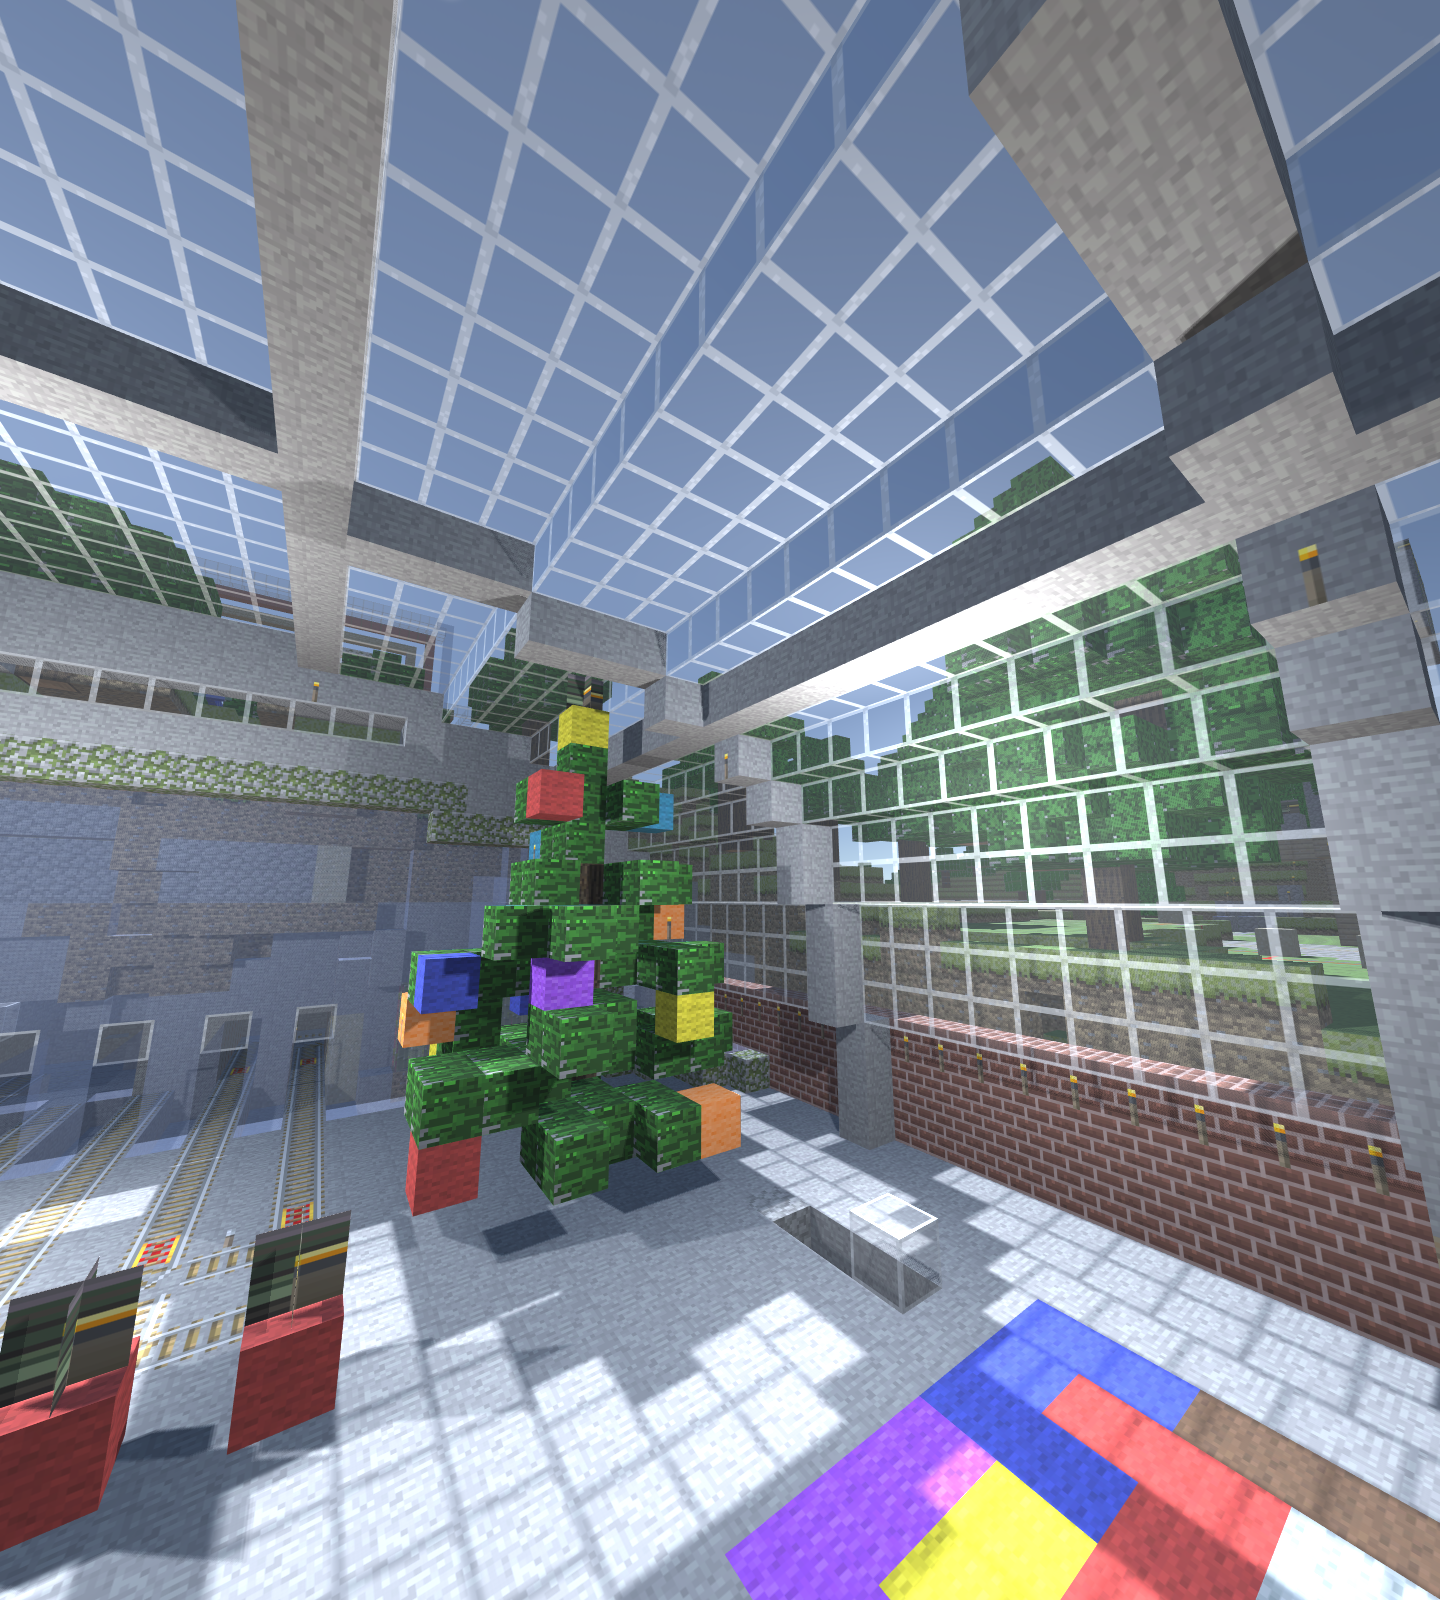
\includegraphics[width=0.96\linewidth]{TOG/figs/mc_gt3.png}}
        
        \subfloat[bedroom scene(\textbf{GT})]{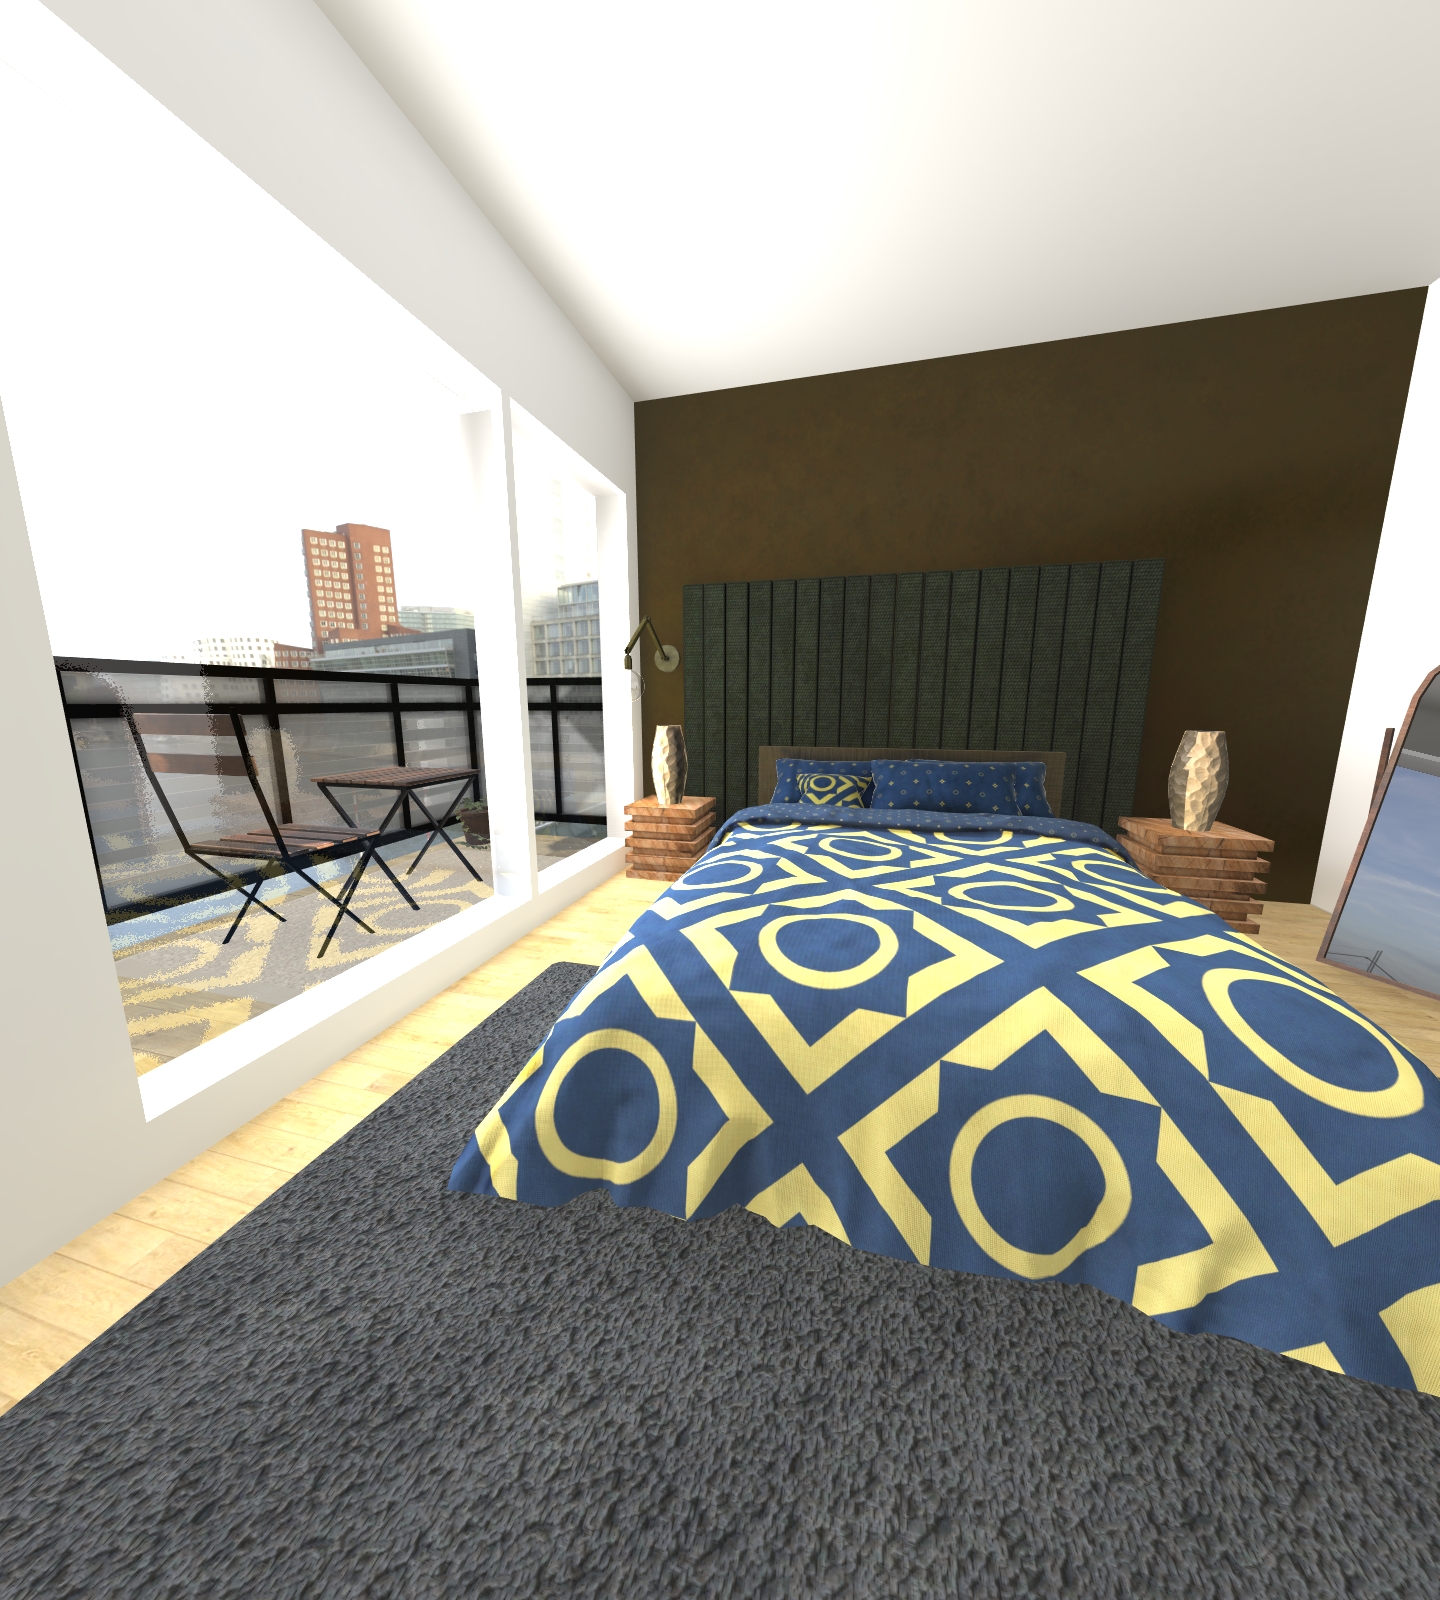
\includegraphics[width=0.96\linewidth]{TOG/figs/bed_gt0.png}}
    \end{minipage}
    \begin{minipage}{0.32\linewidth} %ours
        \subfloat[gas scene (\textbf{OUR})]{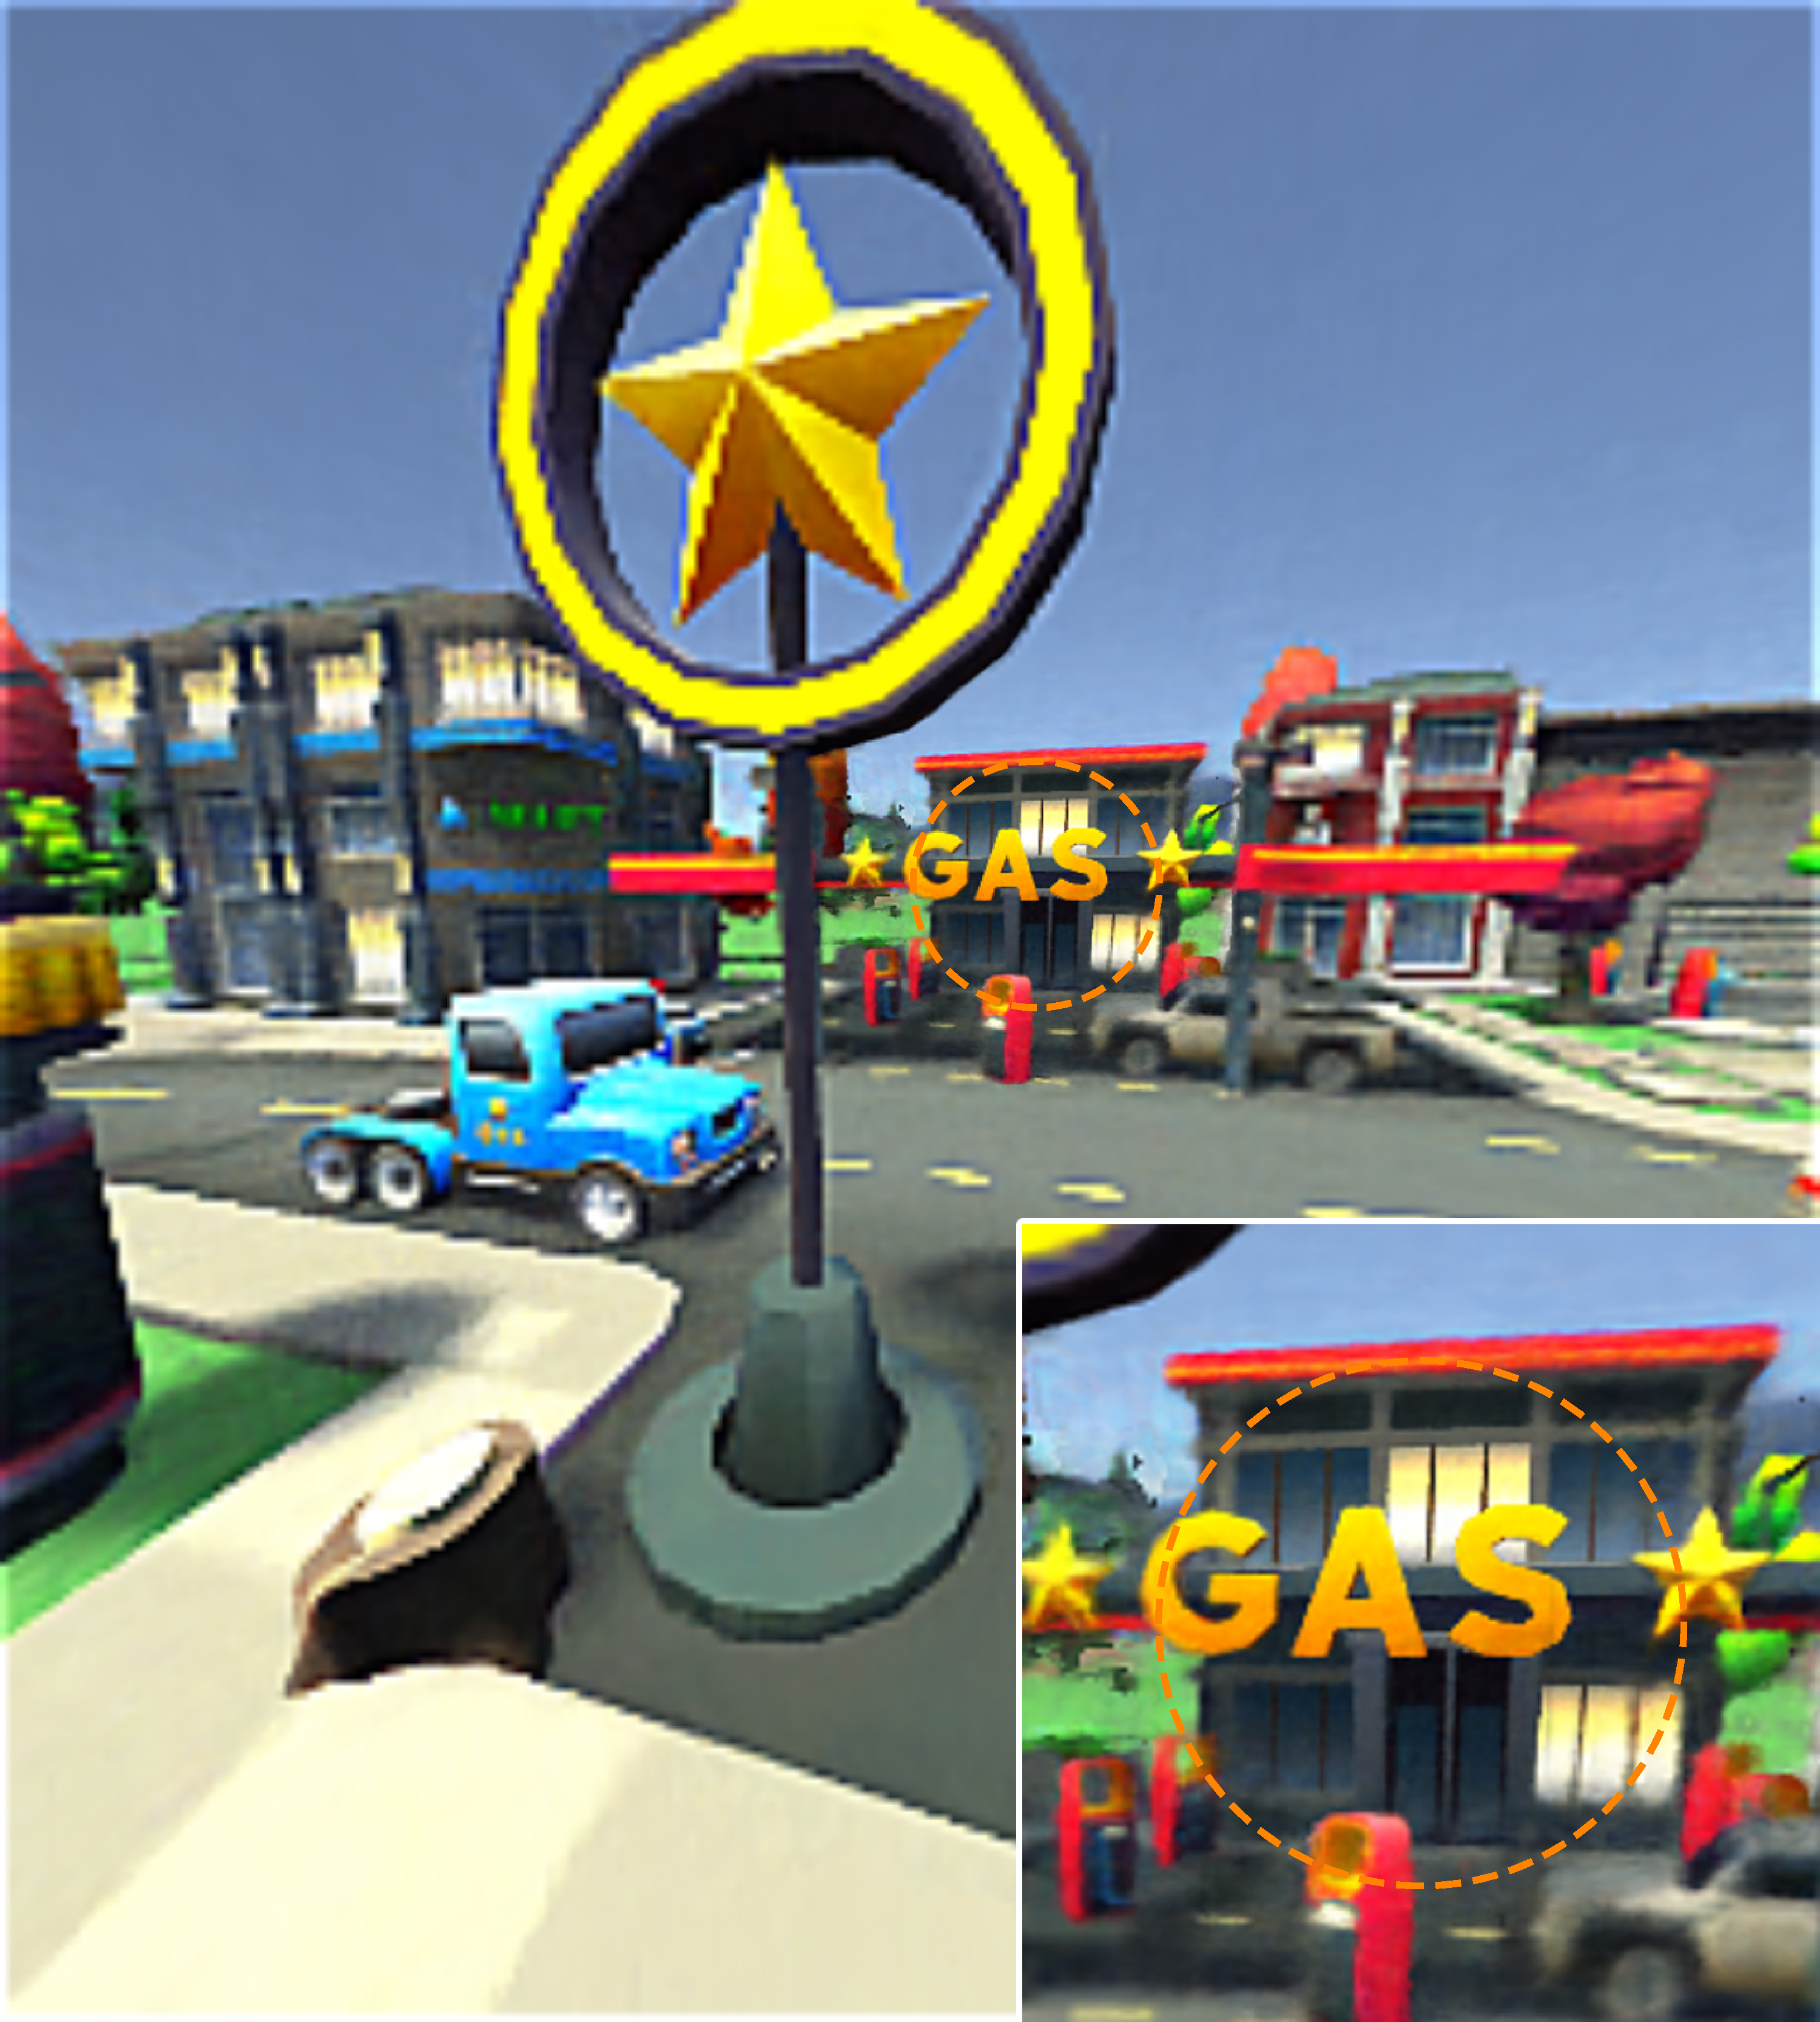
\includegraphics[width=0.96\linewidth]{TOG/figs/gas_our4_inset.pdf}}
        
        \subfloat[minecraft scene (\textbf{OUR})]{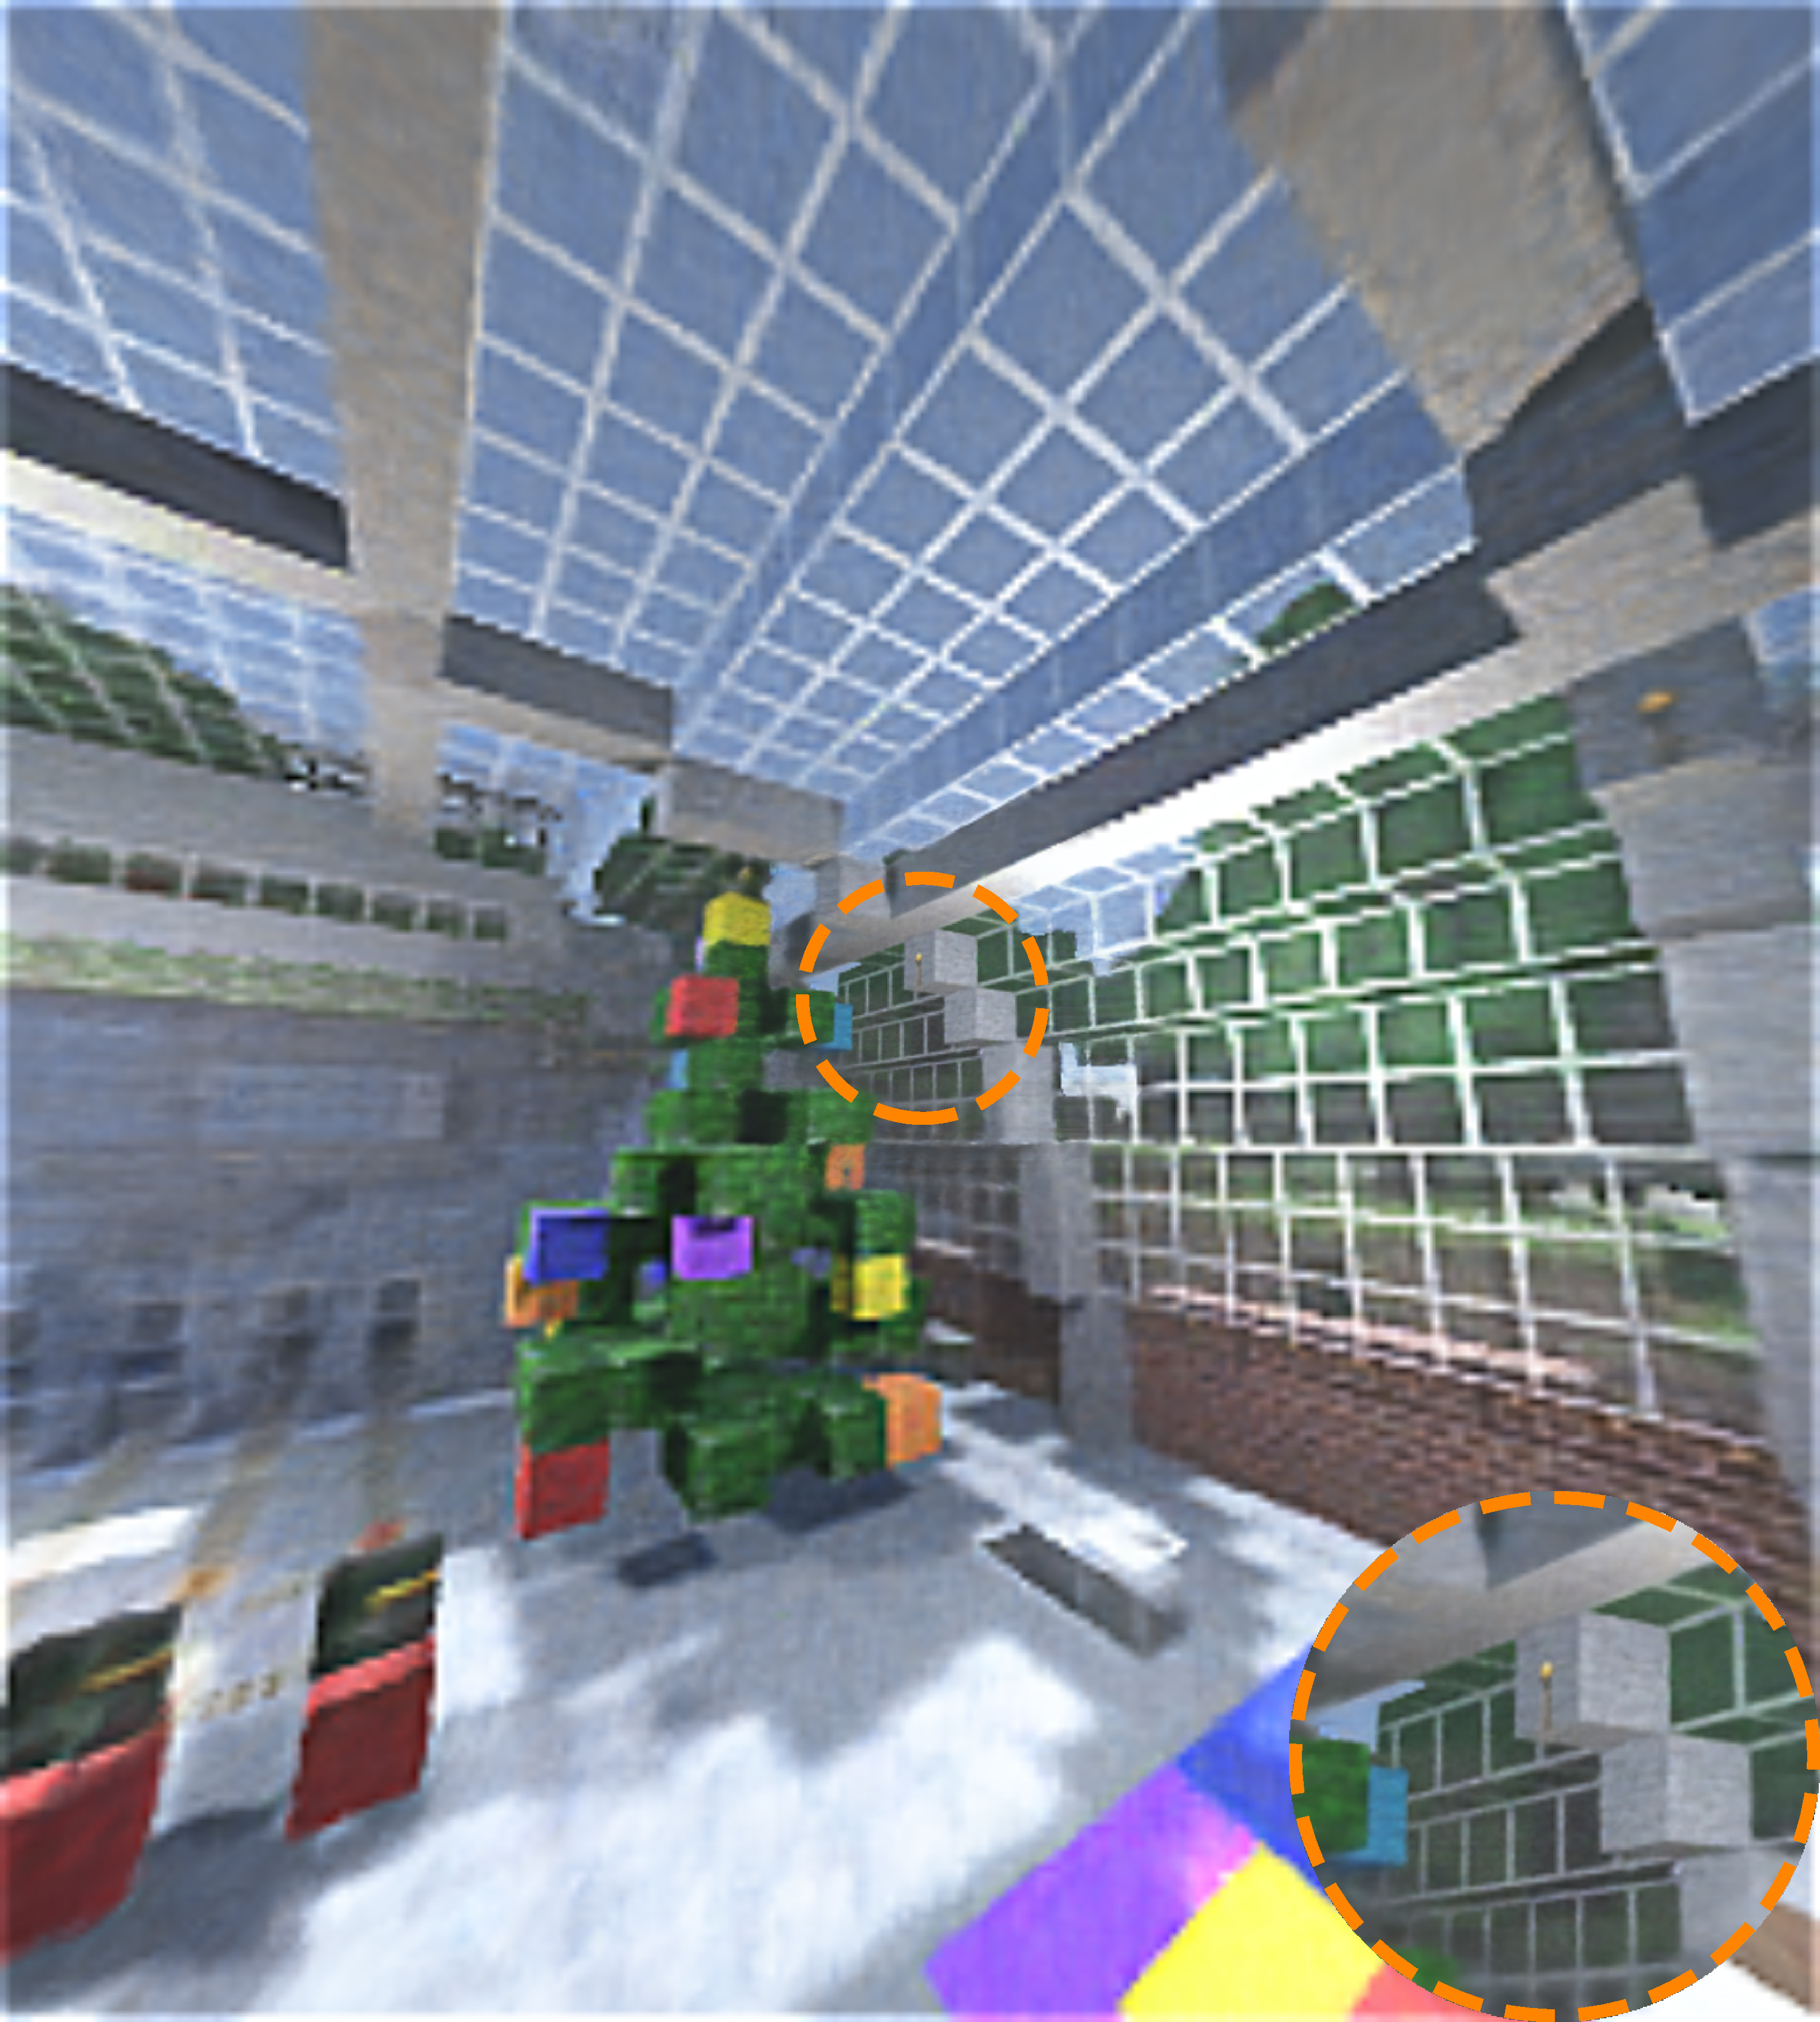
\includegraphics[width=0.96\linewidth]{TOG/figs/mc_our3_inset.pdf}}
        
        \subfloat[bedroom scene (\textbf{OUR})]{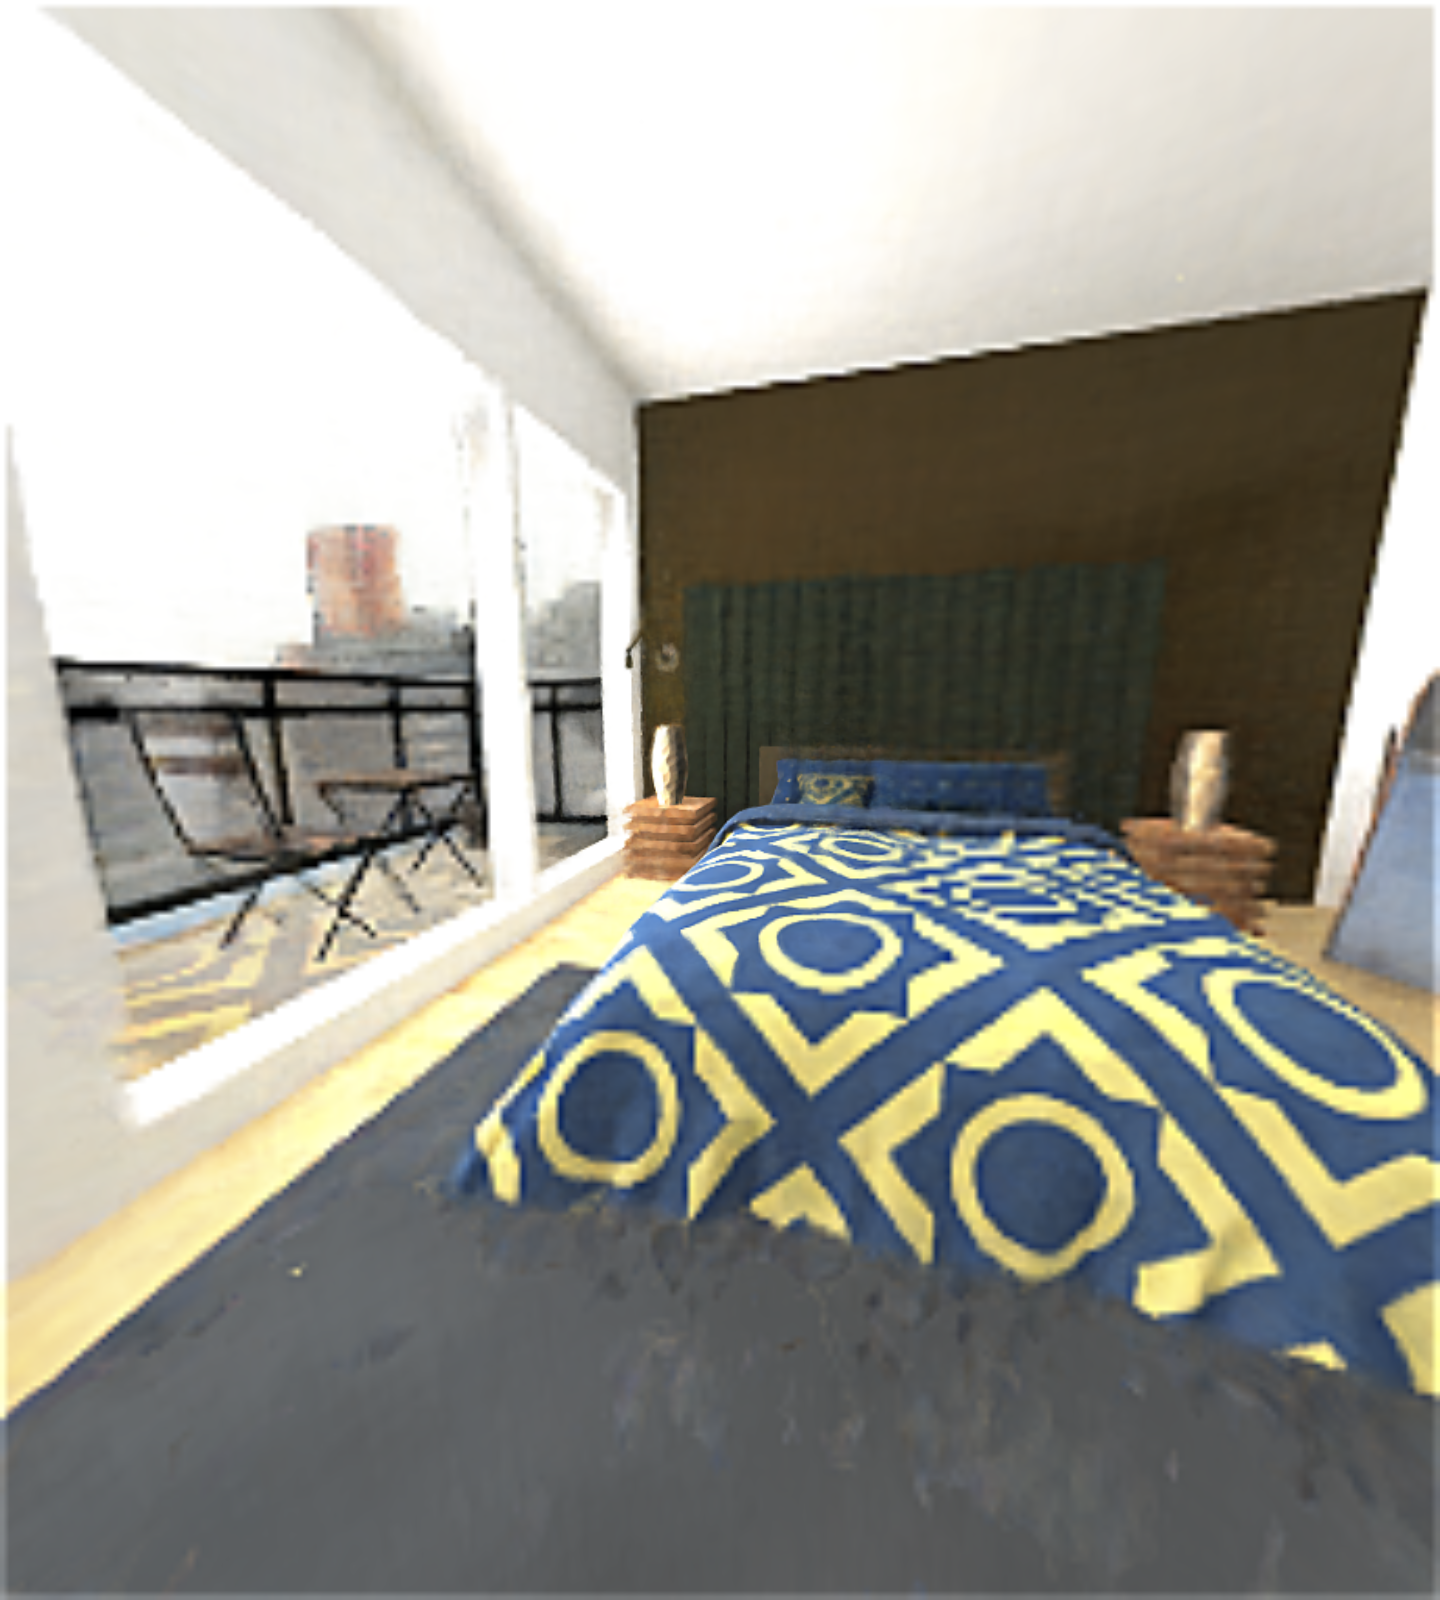
\includegraphics[width=0.96\linewidth]{TOG/figs/bed_our0.png}}               
    \end{minipage}
    \begin{minipage}{0.32\linewidth} % NERF
        \subfloat[gas scene (\textbf{NeRF})]{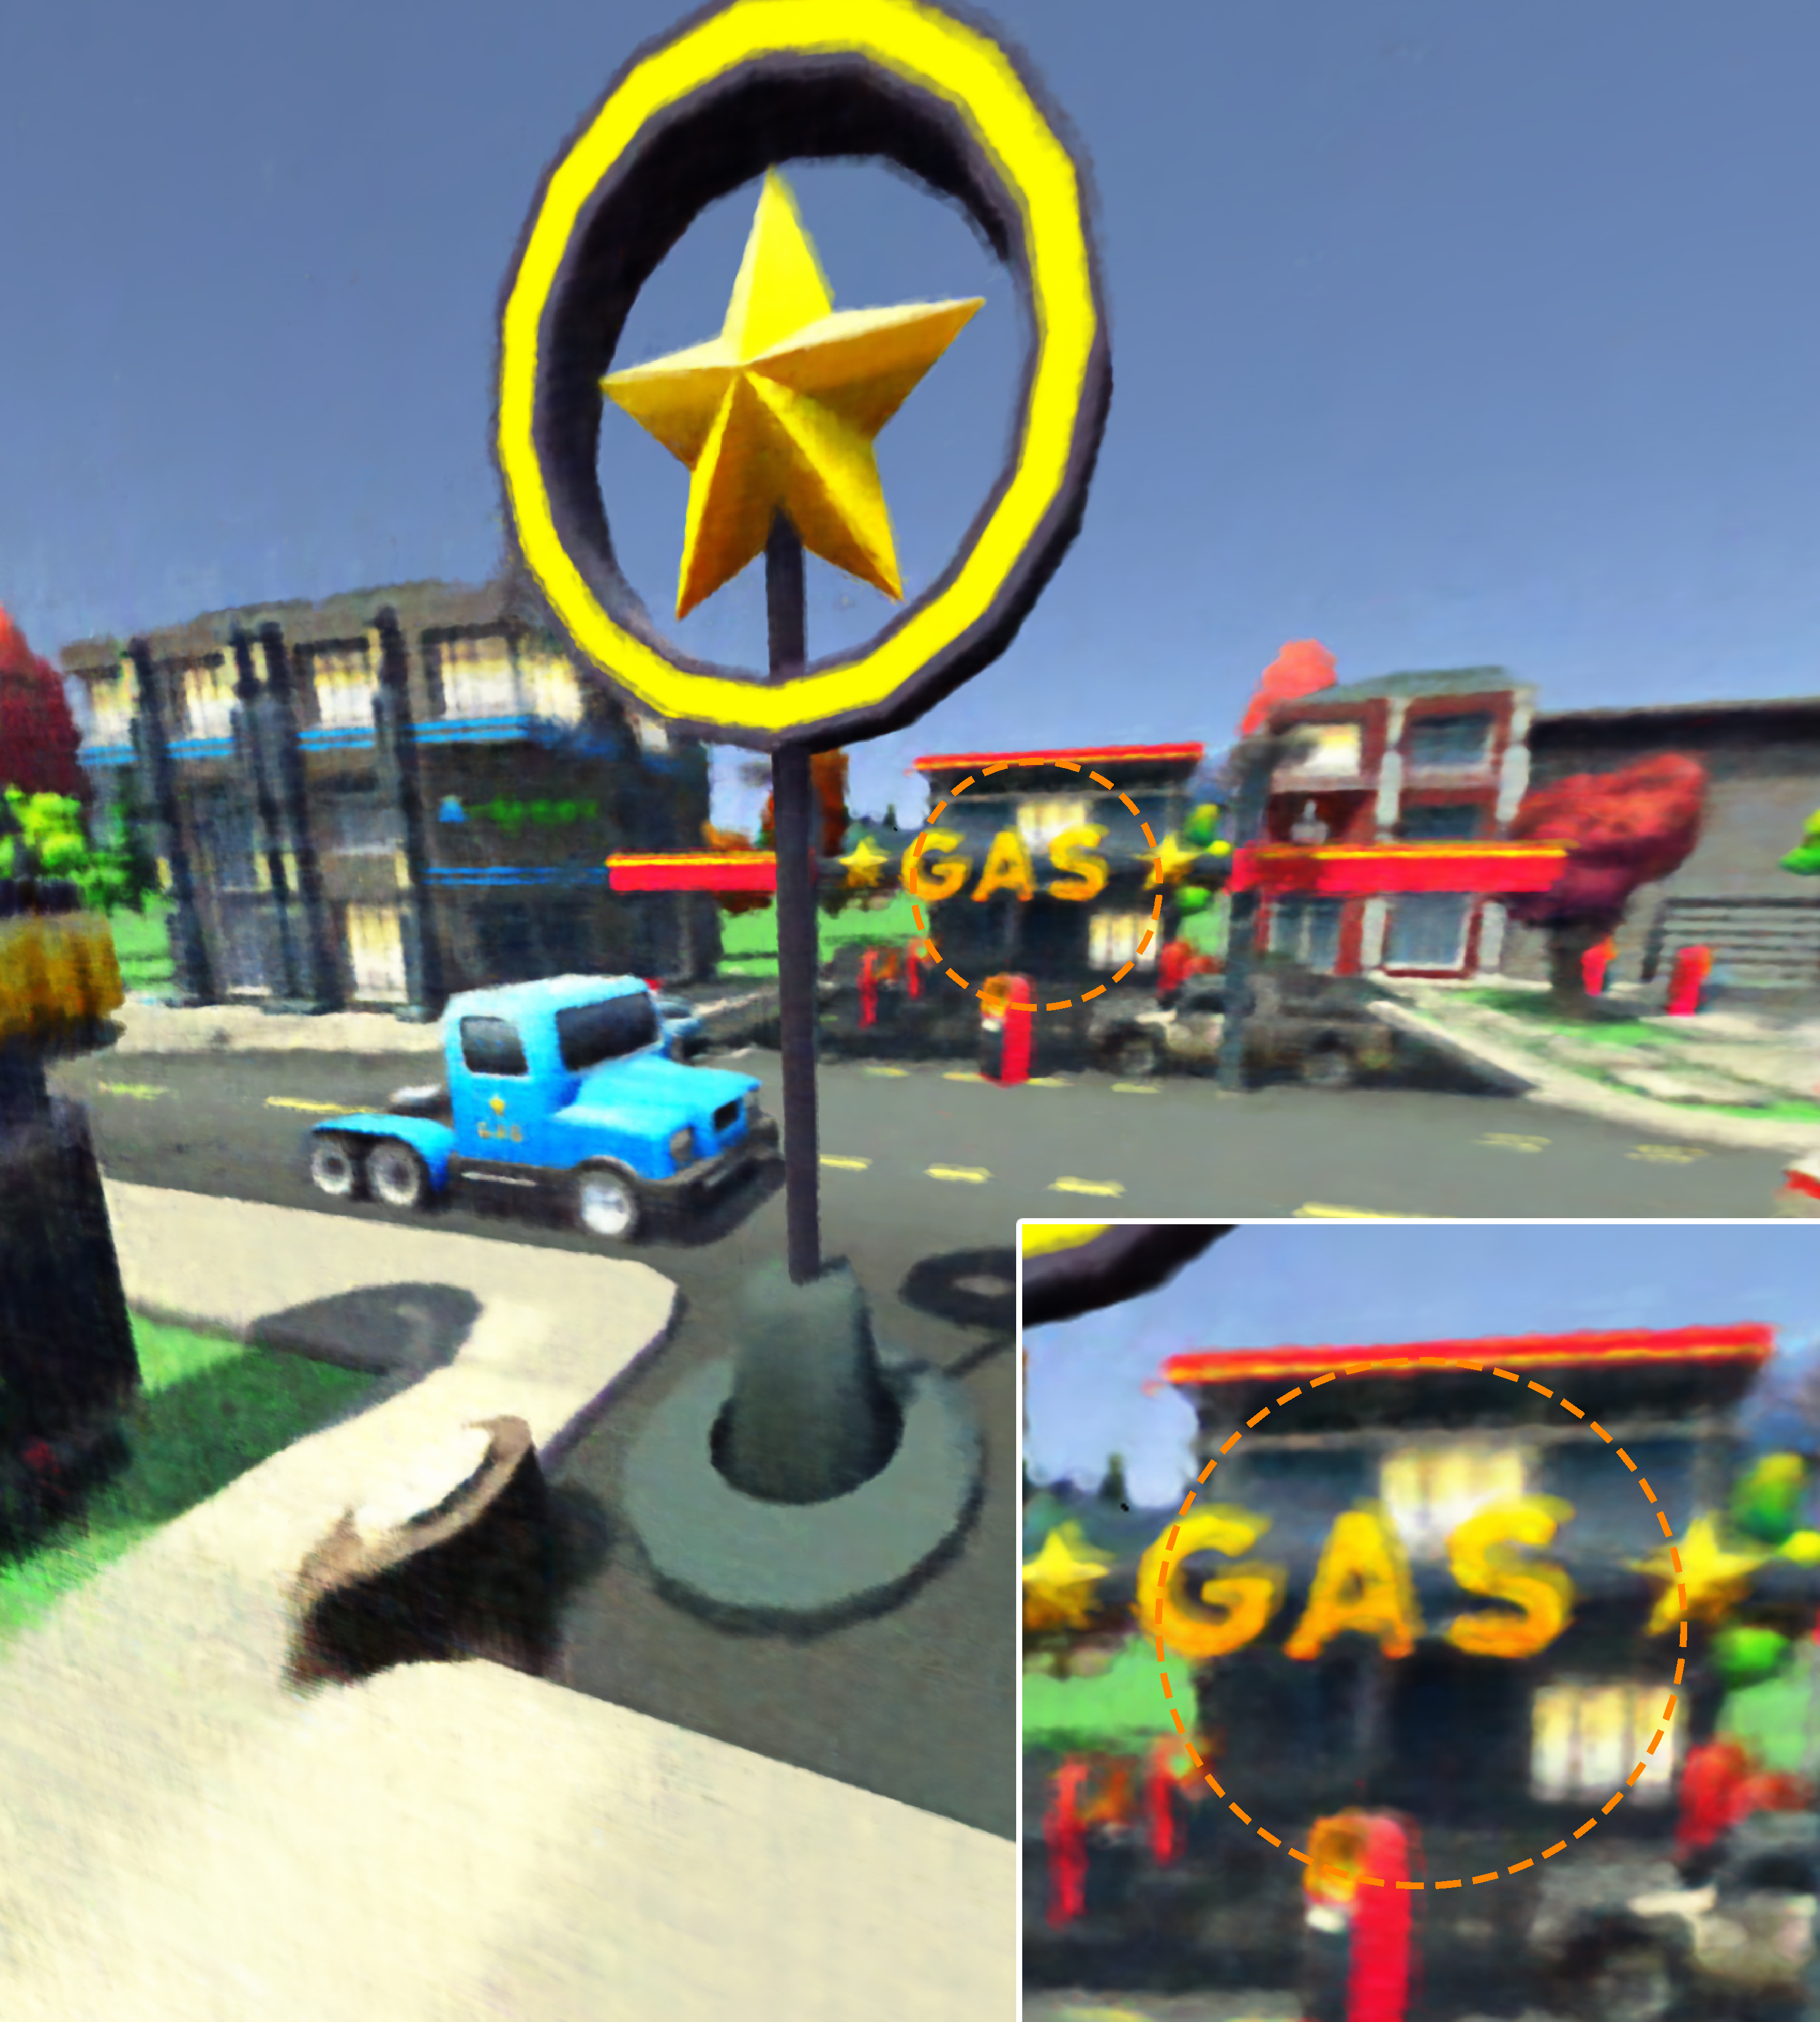
\includegraphics[width=0.96\linewidth]{TOG/figs/gas_nerf4_inset.pdf}}
        
        \subfloat[minecraft scene (\textbf{NeRF})]{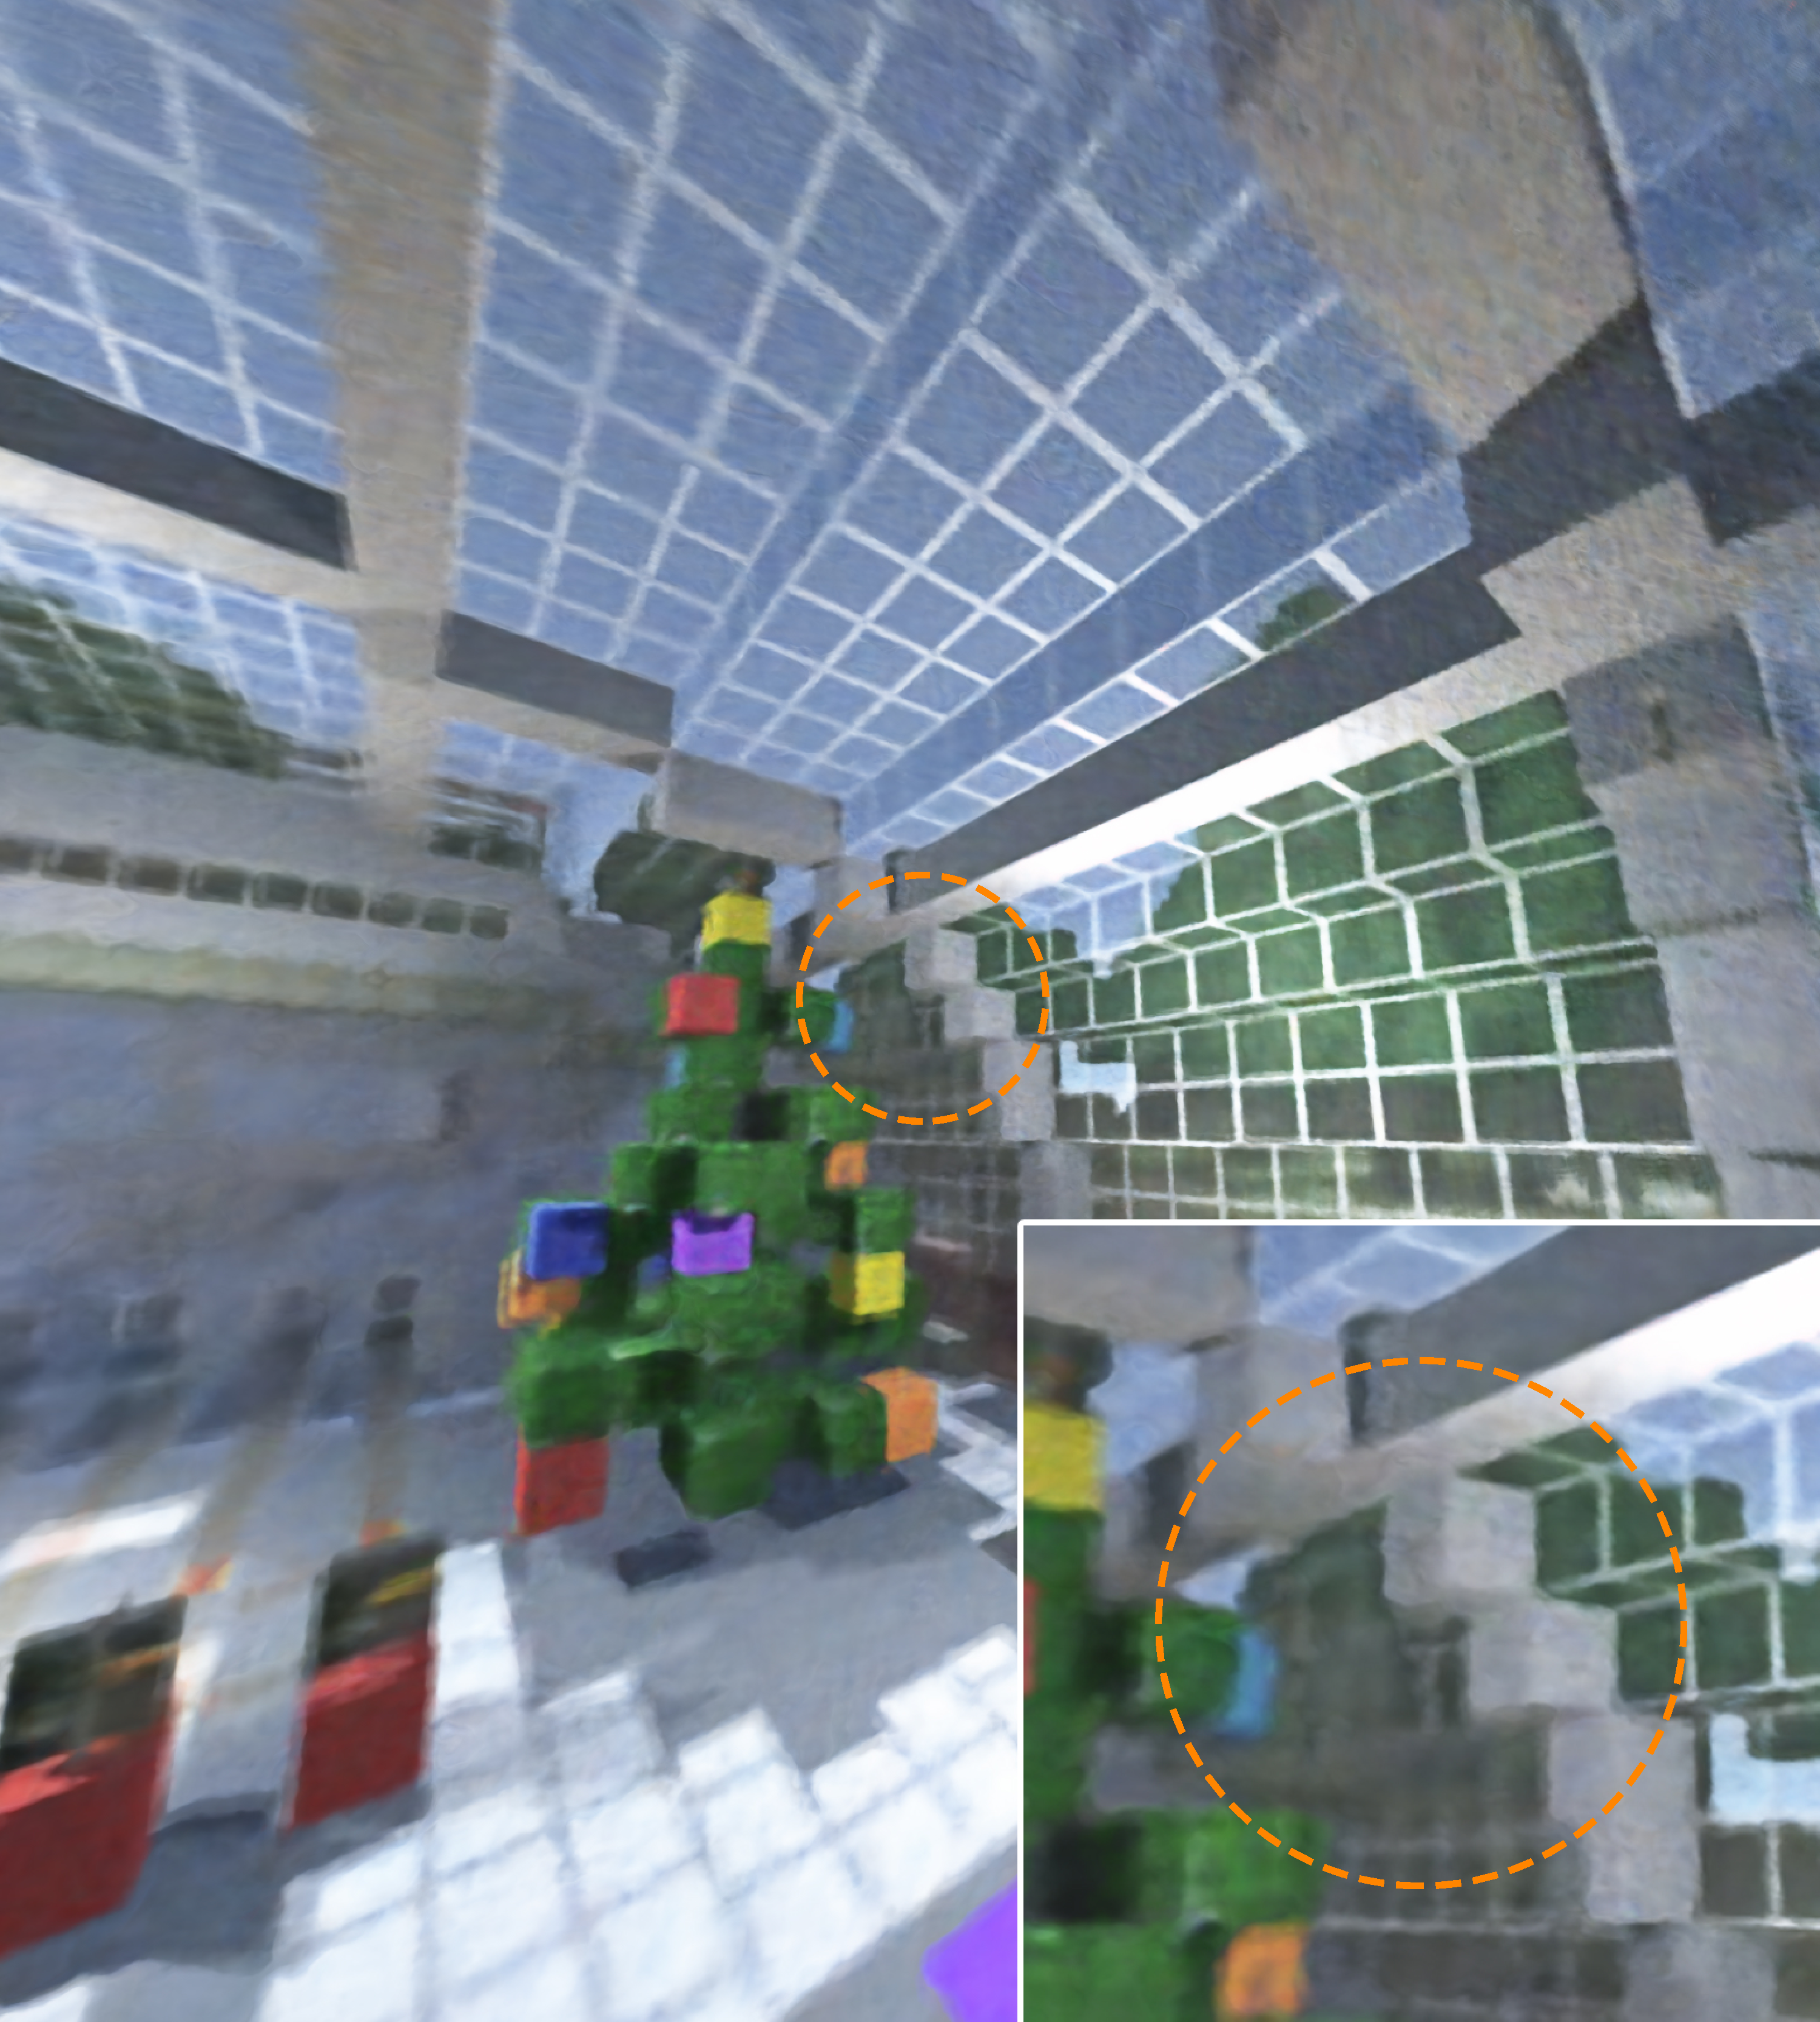
\includegraphics[width=0.96\linewidth]{TOG/figs/mc_nerf3_inset.pdf}}
        
        \subfloat[bedroom scene (\textbf{NeRF})]{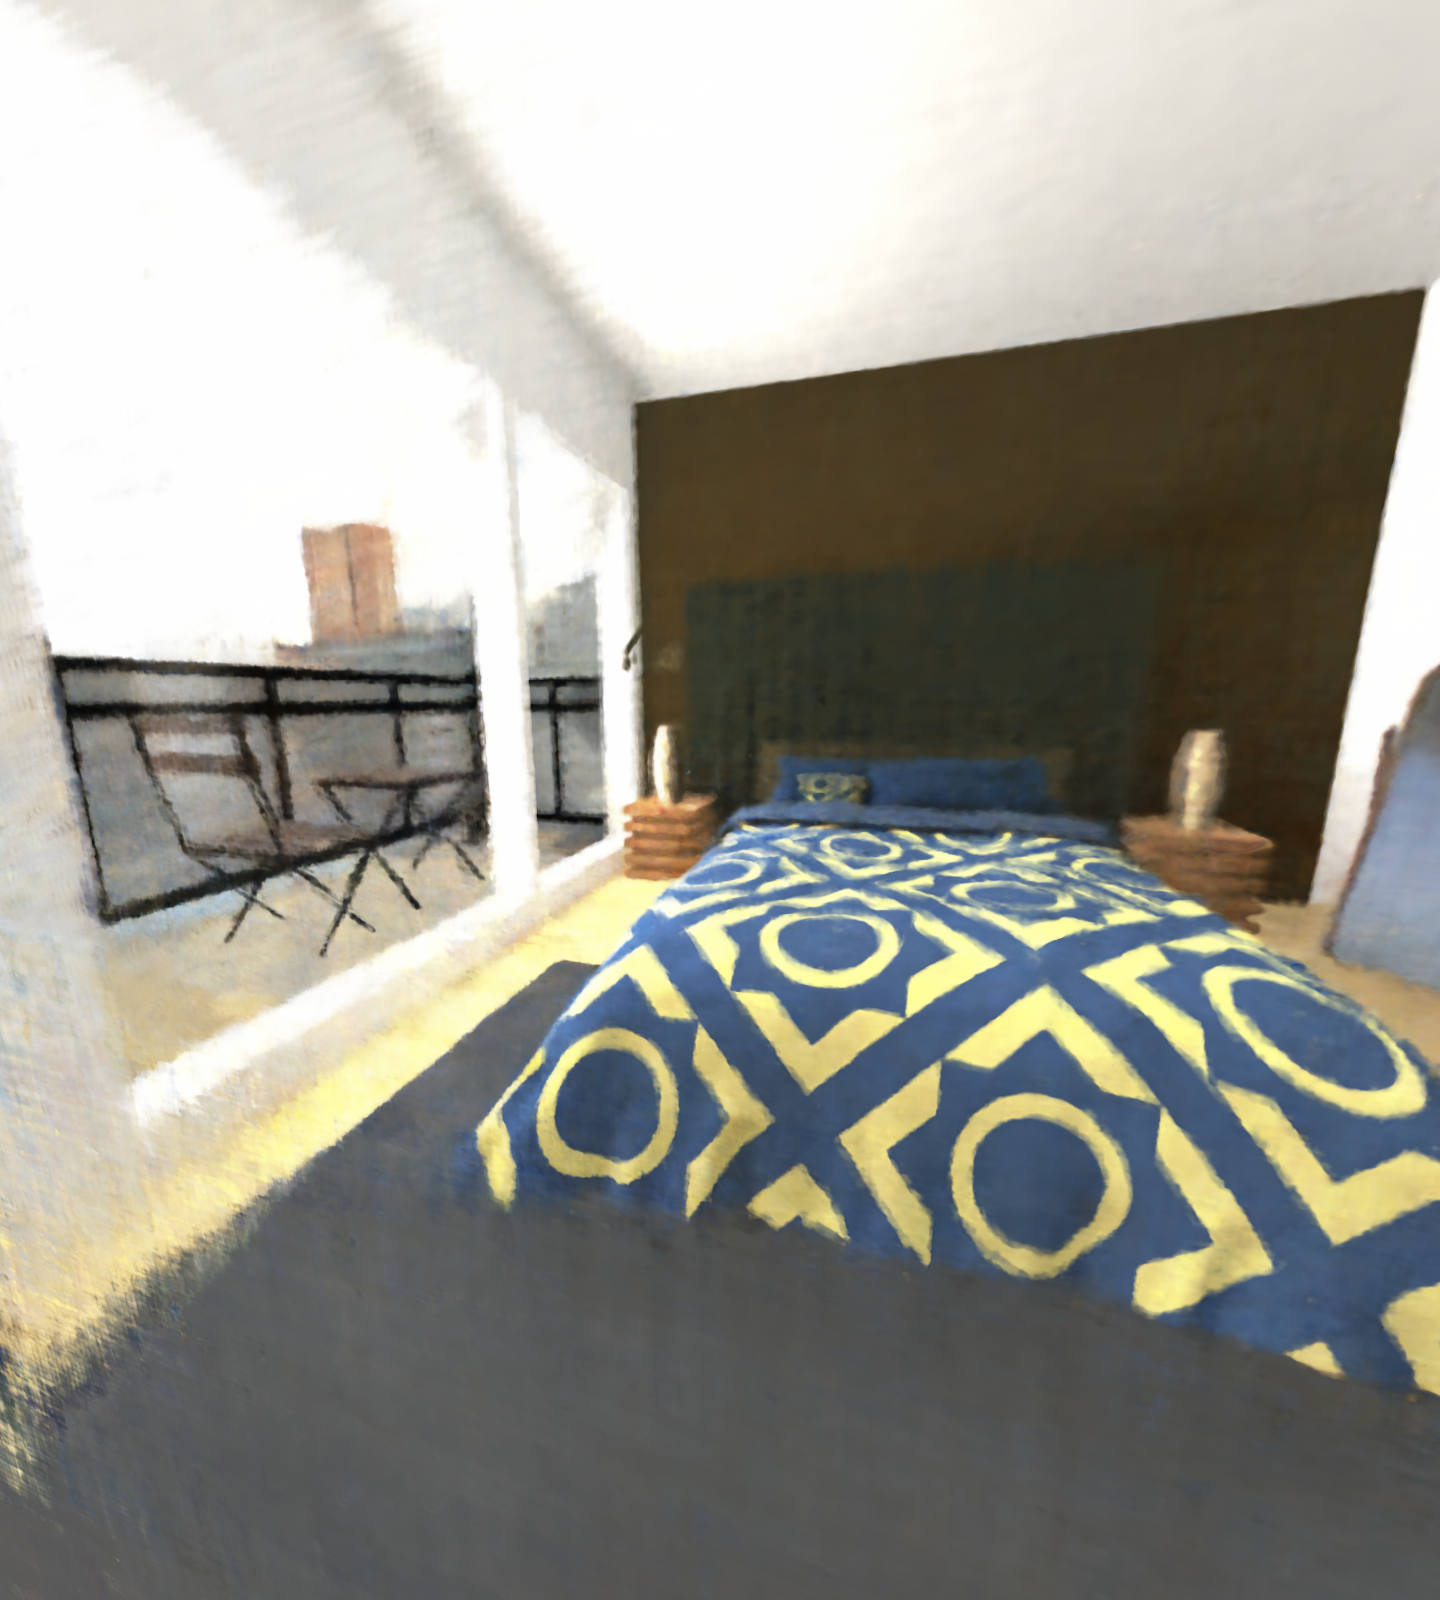
\includegraphics[width=0.96\linewidth]{TOG/figs/bed_nerf0.png}}      
    \end{minipage}    
    
    \caption{Comparing our synthesis method (2nd column) with full resolution (1st column) rendering and NeRF (3rd column).}
    % {\zh{add inset for 2nd and 3rd col}}
    \label{fig:results:comparison}
\end{figure*}

\begin{figure*}[htb]
    \centering
    \begin{minipage}{0.32\linewidth} %full res
        
        \subfloat[gallery scene (\textbf{GT})]{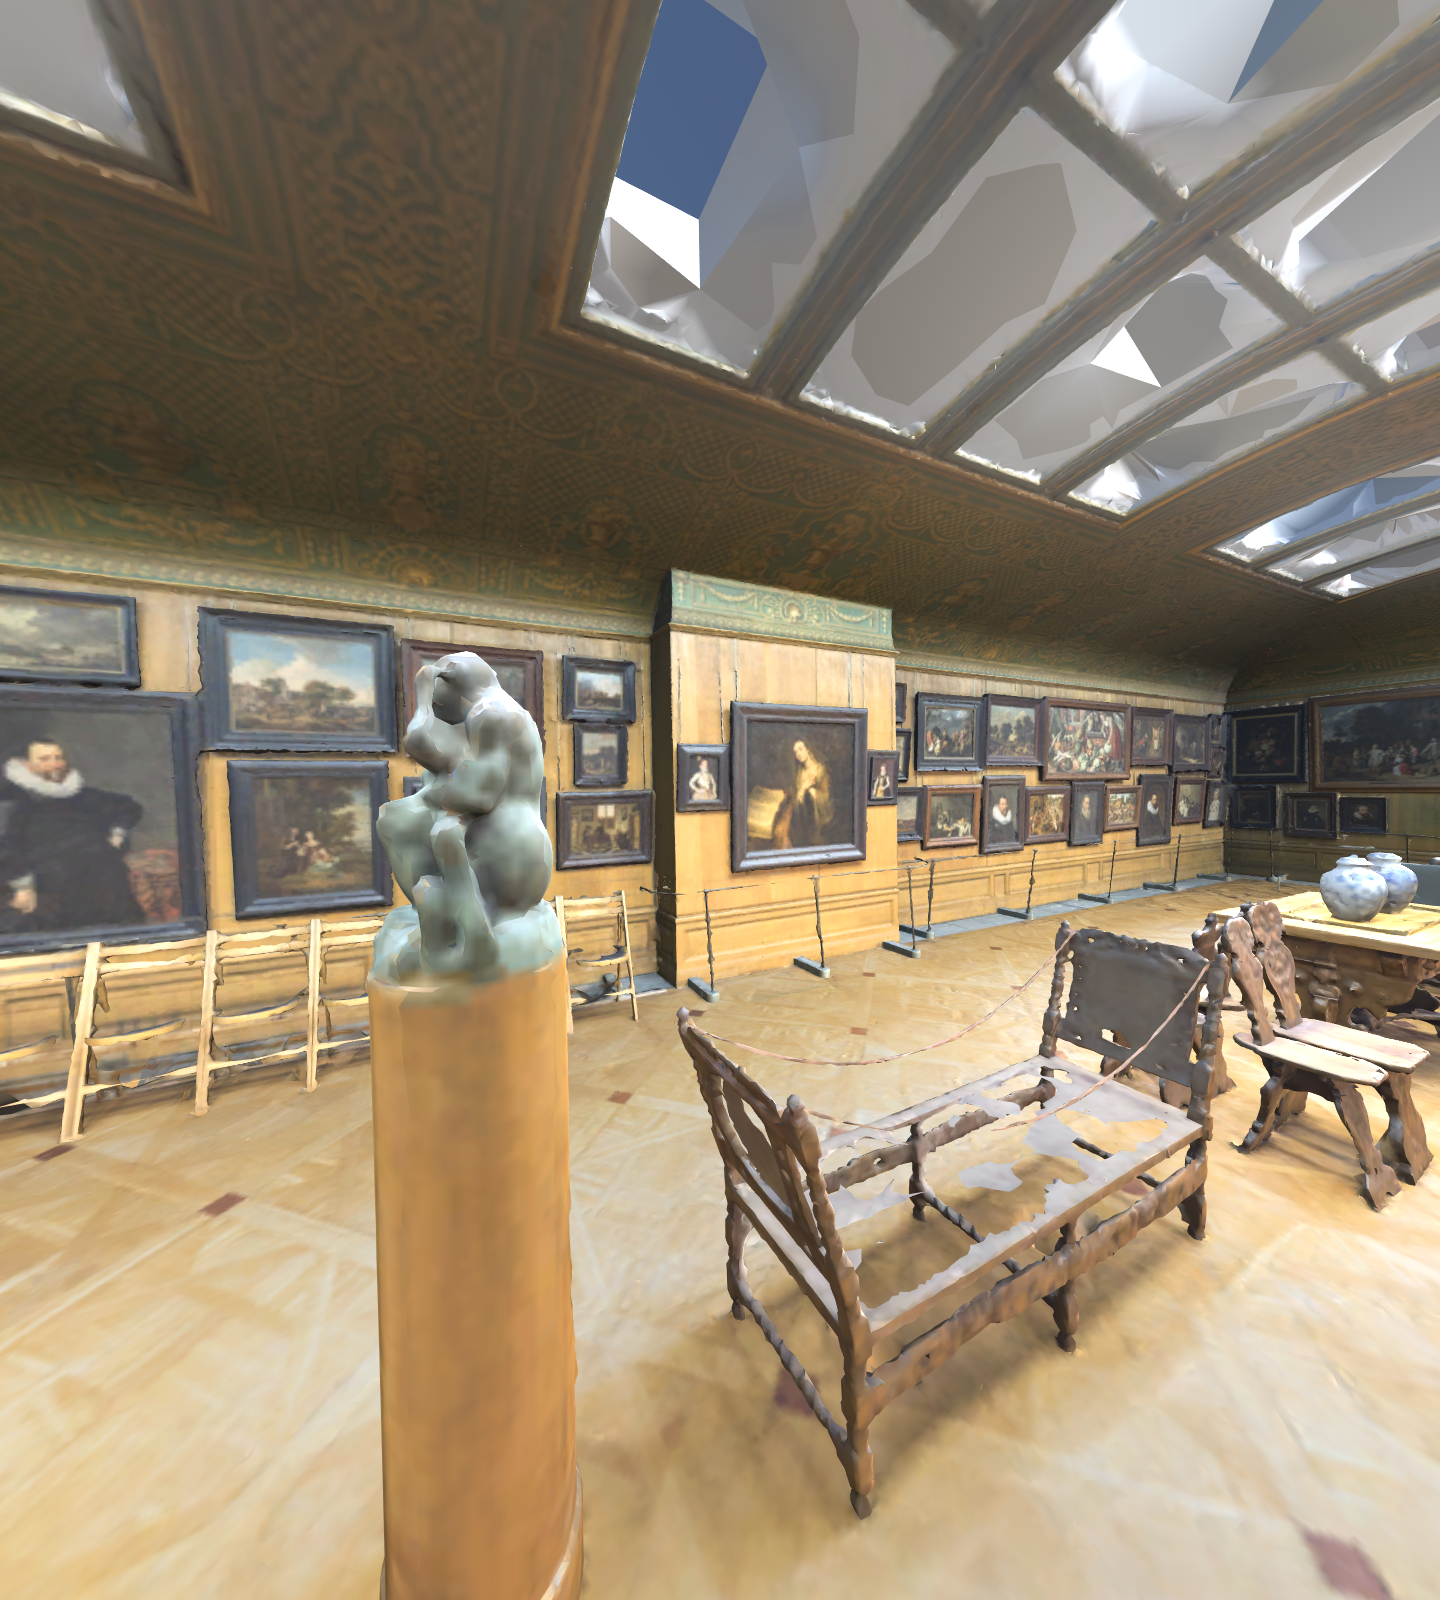
\includegraphics[width=0.96\linewidth]{TOG/figs/gallery_GT_view_0001.png}}
    \end{minipage}
    \begin{minipage}{0.32\linewidth} %ours
        
        \subfloat[gallery scene (\textbf{OUR})]{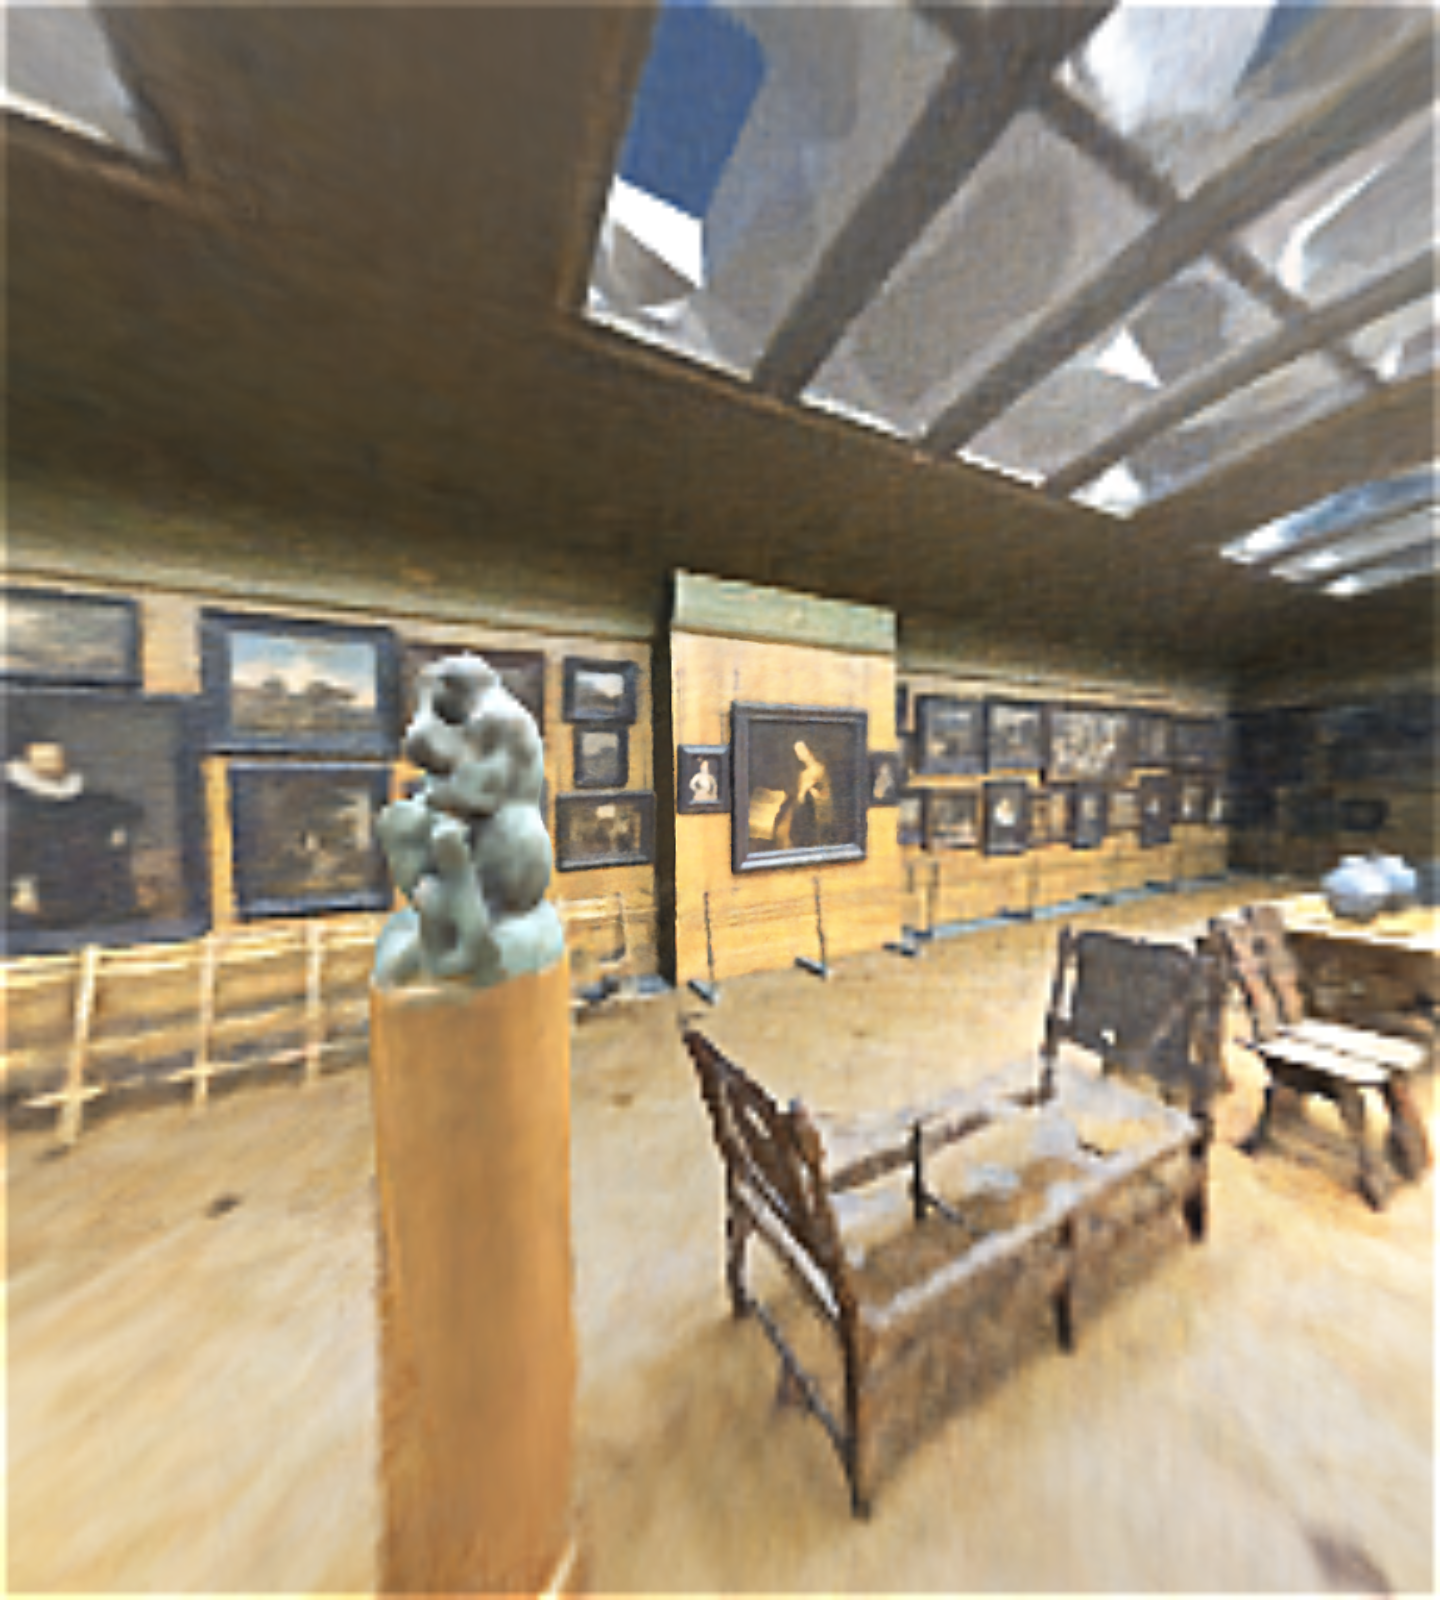
\includegraphics[width=0.96\linewidth]{TOG/figs/gallery_our_001.png}}                
    \end{minipage}
    \begin{minipage}{0.32\linewidth} % NERF
        
        \subfloat[gallery scene (\textbf{NeRF})]{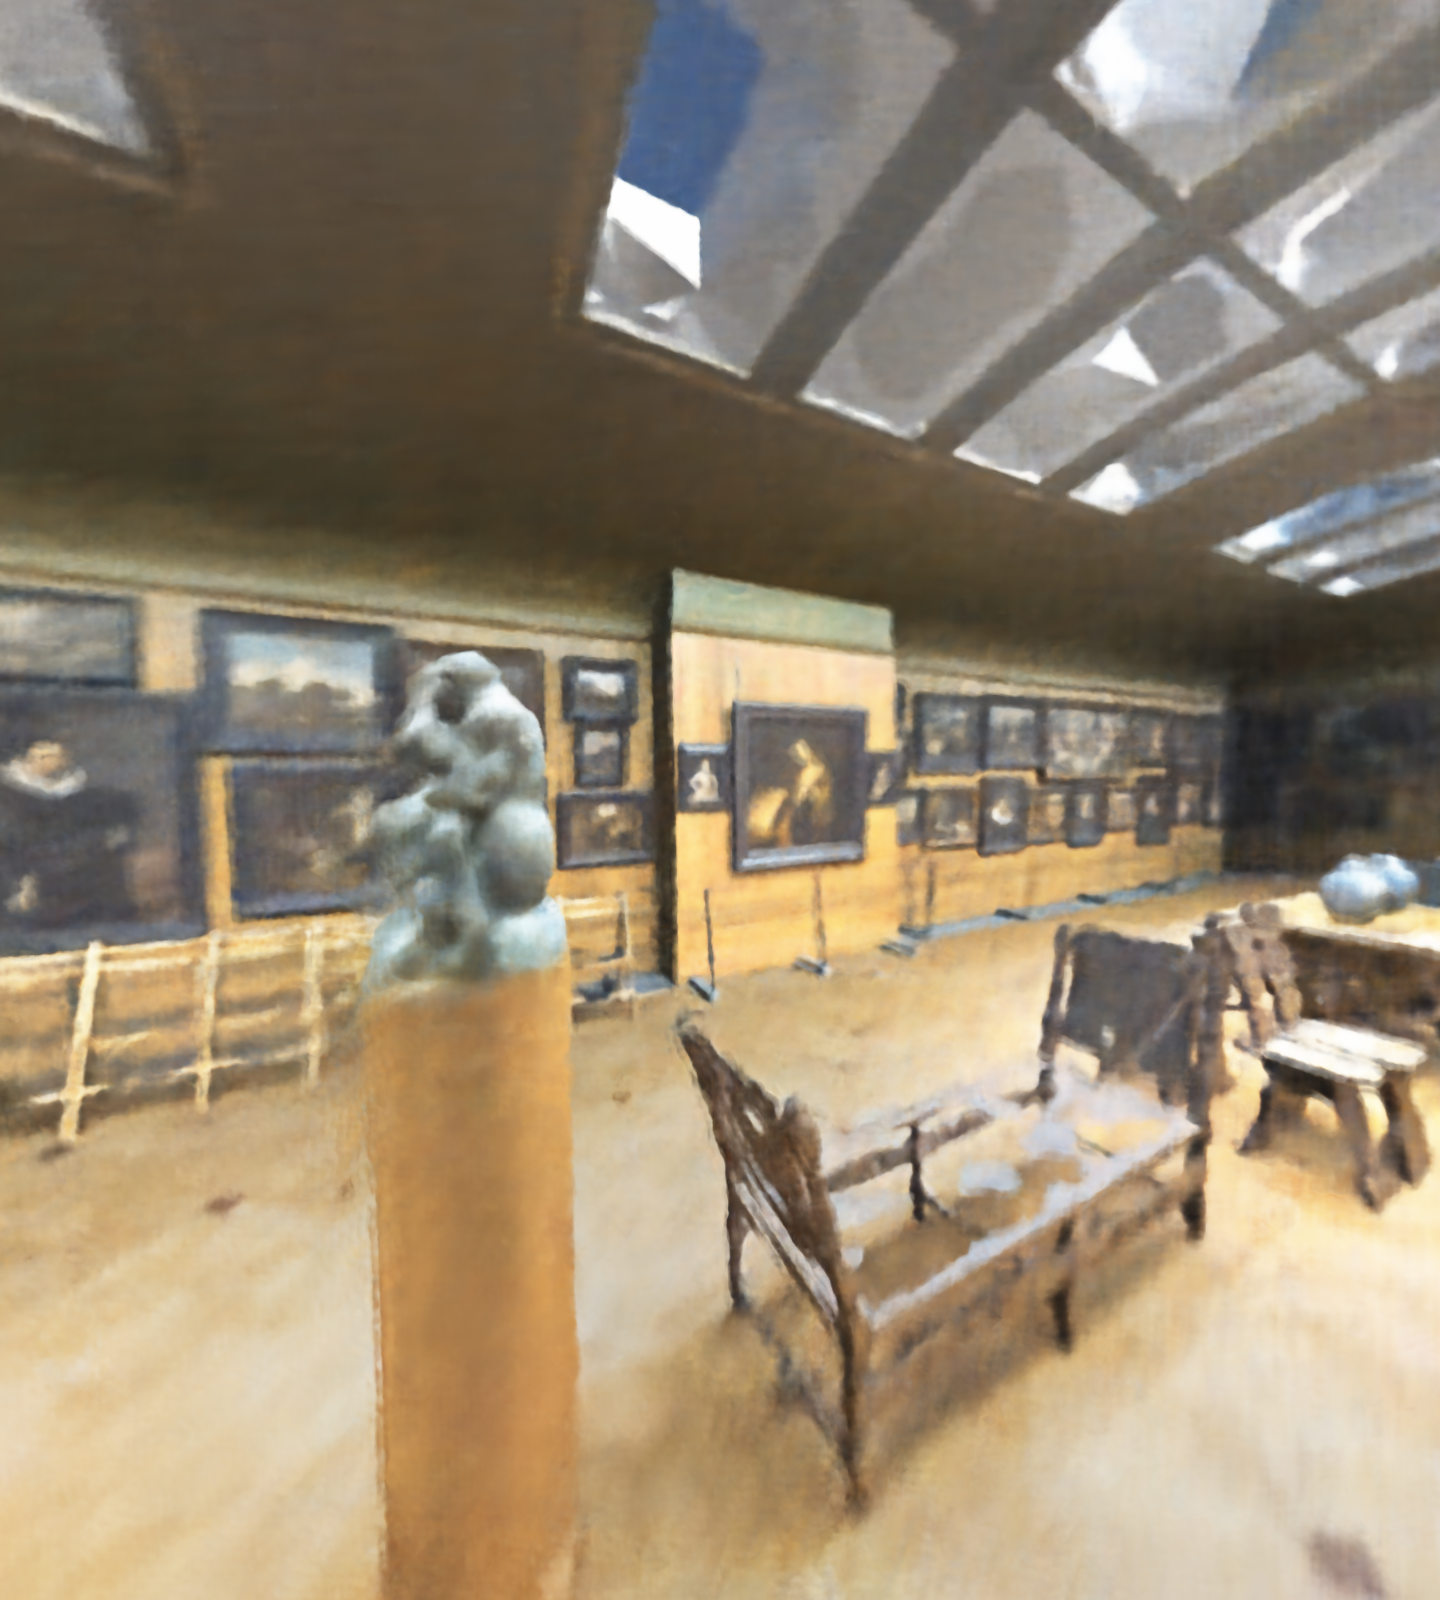
\includegraphics[width=0.96\linewidth]{TOG/figs/gallery_NeRF_001.png}}        
    \end{minipage}    
    
    \caption{Comparing our synthesis method (2nd column) with full resolution (1st column) rendering and NeRF (3rd column). (Cont.).}
    % {\zh{add inset for 2nd and 3rd col}}
    \label{fig:results:comparison2}
\end{figure*}

\subsection{User Study}
\label{sec:study:user}
% \zh{(Jan 10) all the Qs are answered offline, will update the section soon.}

% In this section, we report two perceptual experiments to investigate 1) how users perceive our solution and the ground truth and 2) how our solutions behaves compared to other alternatives.
We first conducted a perceptual experiment to investigate how users perceive our solution ({\bf OURS}) compared to existing solution (\cite{mildenhall2020nerf}, {\bf NeRF}) and original mesh with foveated rendering (\cite{perry2002gaze}, {\bf F-GT}).

% \zh{usually we report the study design here too, like within-subject user study and analyze method, like ANOVA. But I am not sure what we should use here.}
% \zh{(Jan 12), if we include NeRF, I'd say we keep one of the down-sample conditions}

\paragraph{Stimuli}

The stimuli were the images rendered via {\bf F-GT} or synthesized via  {\bf OURS}/{\bf NeRF}, as shown in \Cref{fig:results:comparison}. The resolution of the image per eye was $1440 \times 1600$. 
For fair comparison, each group of stimuli were generated with the same, randomly defined gaze p-osition. The position was indicated as a green cross on the stimuli images.
The resolution of the images per eye was $1440 \times 1600$. 
We used the {\it gas} and {\it minecraft} scenes.
Each condition from individual scene consists of $1$ view and $3$ different gaze positions.

Specifically, we controlled the foveal kernel size in {\bf F-GT} to match our display size and eye-display distances.
For generating {\bf NeRF} condition, we retrained the model from \cite{mildenhall2020nerf} on our dataset with $N_{sample}=16$, $N_{layers}=4$, $N_{channel}=128$. The last column of \Cref{fig:results:comparison} shows the result. 
%We predict the image from the camera transformation, fine-tune the foveated layer, and render the image by alpha blending the three layers.

%\zh{We probably don't need to attach foveated GT here}
% The second column is a uniformly down-sample image at size \warning{??? x ???}. Assuming our network bandwidth is \warning{???}, to stream the images from the cloud in real time, the largest size of the image per eye is up to \warning{??? = ??? / 50 fps / 2 eyes}. So we down sample the entire image with ratio \warning{???}.
%The second column enables foveated rendering. We applied \warning{foveated algorithms} described in \cite{perry2002gaze} and \cite{jiang2015salicon}. 
% and The foveated area is preserved as the original resolution while the rest of the image is down sampled. same alpha blending method that we used in our solution (see \autoref{sec:method:blending}). Similarly, we calculate the size of the foveated image based on the bandwidth. Hence the down-sample ratio of peripheral area is \warning{???}. 
%The third column is generated by NeRF implementation. We retrained a new model on our dataset with parameters $N_{sample}=16$, $N_{layers}=4$, $N_{channel}=128$. The last column is our result. We predict the image from the camera transformation, fine-tune the foveated layer, and render the image by alpha blending the three layers.

\paragraph{Setup}
Each participant was asked to wear a eye-tracked HTC Vive Pro Eye headset during the experiment. During the experiment, the participants wearing the headset examining  the stimuli. 
Fourteen users participated in the study and 13 of them managed to complete (4 females and 9 males, $M=23.08$, $SD=1.75$). One participant (age=23, female) did not complete the experiment due to gaze drifting (please refer to the task description below).
None of the subjects were aware of the research, the experimental hypothesis, or the number of rendering methods. All participants had normal or corrected-to-normal vision.

\paragraph{Task}
The task was a \textit{two-alternative-forced-choice} (2AFC). Each trial consists of a pair of stimuli from the three conditions ({\bf OURS} / {\bf NeRF} / {\bf F-GT}). Each stimulus appeared for $300$ms on the the display. A forced $1.5$sec break was introduced between conditions. During the study, the participants were instructed to fix their gazes on the green cross. To prevent fixation from shifting away, we tracked the users gaze during the whole experiment. Whenever the gaze is $1$deg away from the target, a trial was dropped immediately with black green informing the participant.
After each trial, the participants were instructed to select which one of the two stimuli appeared with higher visual quality using keyboard.
Before each experiment, a warm-up session with 1 trial was provided to have the participants familiarize the study procedure. The order of conditions cmong trials were randomized with counterbalancing.
%To start with, each participant was informed that they were required to choose an alternative with higher quality after watching each pair of stimuli. We calibrated the device and performed a warm-up trial to help participants understand our system. Each participant were provided with 1 warm-up trial and 6 official trials (2 scenes x 1 view x 3 gaze positions) where each trial consisted all the combinations of the pairs of every two stimuli. We randomize the order of the pairs for counterbalancing. We showed a yellow cross on the screen. After participants move their gaze positions to the area close to the cross, the yellow cross turns green. The first stimulus will be rendered as well as the cross after participants fixate the cross for 1 second. Each stimulus is displayed for 300 milliseconds. The second one will be rendered after 1.5-second dark screen. If the participants does not fixate at the cross when stimuli are displayed, the current pair will be discarded and displayed to the participants later in the same trial. After each pair, participants reported their opinions on which image has higher quality.
To minimize the effect of accumulating discomfort during the experiment, we enforced at least a 60-second break between each trial. Meanwhile, the participants were instructed to take as much time as needed to recover. 

\paragraph{Results}
\Cref{fig:results:2afc} plots the study results. 
Among all three conditions, we observed near to random guess among trails that compares  {\bf F-GT} and {\bf OURS} (50.0\% voted for {\bf OURS}). However, participants significantly prefers  {\bf F-GT} over {\bf NeRF} (98.7\% voted for NeRF, binomial test showed $p<0.005^{***}$). The preference applies to {\bf OURS} vs. {\bf F-GT} as well (97.4\% voted for NeRF, binomial test showed $p<0.005^{***}$).

% our/gt 78/156 0.5318897993488445
% our/nerf 152/156 2.6681140960754964e-40
% nerf/gt 2/156 1.3407579916082842e-43

\begin{figure}[htb]
    \centering
    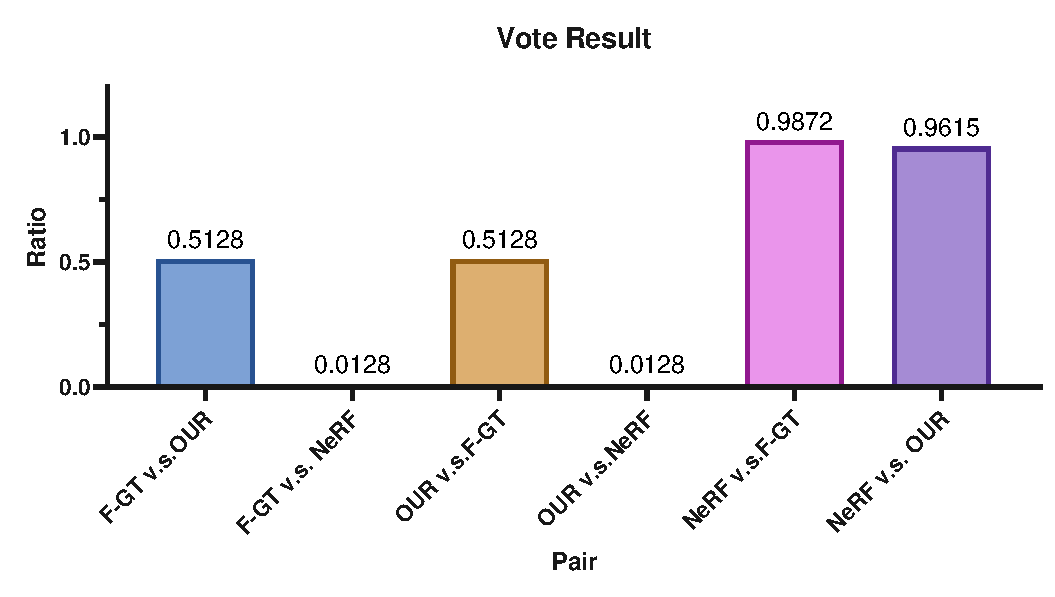
\includegraphics[width=0.96\linewidth]{TOG/figs/vote.pdf}
    \caption{The users' preference votes from our evaluation experiment. X axis shows all the pair combination and Y axis shows the ratio of voting for the second one.}
    \label{fig:results:2afc}
\end{figure}

% apply binomial test https://docs.scipy.org/doc/scipy/reference/generated/scipy.stats.binom_test.html
% or apply ANOVA, there is a value of votes for each condition and we want to know if there exists significant effects on different condition.
\paragraph{Discussion}
The near-to-random-guess indicated the statistically similar perceptual quality between {\bf OURS} and foveated ground truth ({\bf F-GT}). 
Given the perceptual identicality between foveated and full-resolution rendering, the subjective study indicates that {\bf OURS} can achieve similar quality as a rendering with a locally fully stored high-quality mesh.
Meanwhile, both of the two conditions showed significant subjective quality preference than {\bf NeRF}. That is, under an immersive, high FoV, and first-person view, the current volume-based scene representation may not fully reproduce the perceptually identical retinal images.
To further validate the perceptual quality by breakdown across the whole visual field, we conducted measurements with objective metrics in the following section.

\subsection{Visual Quality}
\label{sec:study:quality}
Complementary to the subjective measurement (\Cref{sec:study:user}), we evaluate the perceived quality in an objective fashion. Specifically, under four different scenes (indoor/outdoor, artificial/realistic), we compare {\bf OURS}, {\bf F-GT} and {\bf NeRF} at individual eccentricity ranges across the whole visual field (up to $110$ deg, the capability of the VR HMD). 
%\zh{gonna comment this: To validate the non-uniform perceptual quality on the retina, we apply a foveated filtering to {\bf GT} \cite{perry2002gaze,jiang2015salicon}.}
For each eccentricity range, we compare the deep perceptual similarity (LPIPS) \cite{zhang2018unreasonable} across all scenes. LPIPS uses deep neural networks to evaluate perceptual similarity between the image provided and a reference image. Smaller values indicate higher perceptual similarity.
For each scene, we sample $20$ views with gazes at the middle of the display, resulting in $20$ data per eccentricity value, $420$ data per scene. We used one-way repeated measures ANOVAs to compare effects across three stimuli on each eccentricity value and together. Paired t-tests with Holm correction were used for all pairwise comparisons between stimuli. All tests for significance were made at the $\alpha=0.05$ level. 
% The error bars in the graphs show the 95\% confidence intervals of the means.

\paragraph{Results} 
\Cref{fig:lpips} plots LPIPS values across all scenes and eccentricity ranges ($5$ deg per sample). 
From foveal to near periphery (<=$40$ deg), we observed significant effects of the stimuli on LPIPS with a ``large'' effect size ($\eta^2 = 0.84$). That is, \textbf{OUR} shows significantly lower LPIPS than \textbf{NeRF} ($p<.001^{***}$), while significantly higher LPIPS than \textbf{F-GT} ($p<.001^{***}$).
For example, the main effects of stimuli ($F(2,38)=42.023, p=.001^{***}$) was significant on eccentricity $=25$  deg  in scene \textit{gas} (\Cref{fig:lpips:gas}). \textbf{OUR} was significantly lower than \textbf{NeRF} ($t(19)=-18.557, p<.001^{***}$) and \textbf{F-GT} ($t(19)=-10.342, p<.001^{***}$) both with a ``large'' effect size (Cohen's d $>0.8$). 

From mid- to far- periphery (>$40$ deg ), we observed significant effects of the stimuli on LPIPS with a ``large'' effect size ($\omega^2 = 0.19$). \textbf{OUR} shows significantly higher LPIPS than \textbf{NeRF} due to the foveated nature of our design. Whereas, comparing with \textbf{F-GT}, we observed  significant lower scores ($p<.001^{***}$).
For instance, the main effects of stimuli was significant on eccentricity $=60$ deg in scene \textit{gas} ($F(2,38)=493.51, p<.001^{***}$, \Cref{fig:lpips:gas}). \textbf{OUR} was significantly lower than \textbf{F-GT} ($t(19)=-12.28, p<.001^{***}$), and higher than \textbf{NeRF} ($t(19)=18.90, p<.001^{***}$) both with a ``large'' effect size (Cohen's d $>0.8$). 

The general trend applies to all 4 scenes being validated. 

\paragraph{Discussion}
The observation revealed our method's over-performance than alternative view synthesis solutions in the foveal and near peripheral vision. This is evidenced by the significantly increased perceptual similarity to \textbf{GT} while comparing between \textbf{OUR} and \textbf{NeRF}.\zh{``significantly increased LPIPS'' requires analysis}

Meanwhile, \textbf{OUR}'s increased perceptual similarity comparing with \textbf{F-GT} beyond $40$ deg indicated their similar visual quality. This shows that \textbf{OUR} doesn't compromise the peripheral vision's quality with its significantly enhanced foveal image. 

The discoveries also agrees with the trend from \Cref{sec:study:user}. That is, in addition to the faster performance, our method showed remarkably perceptual quality gain than \textbf{NeRF} for first-person 6DoF immersive viewing of 3D scenes: our synthesized views are perceptually identical to the traditionally rendered images from complete mesh. It yet achieves significant data storage saving (\warning{xxx\%-xxx\%}).

% ZH: why \Cref{fig:lpips:gas} shows 'section 5.2'
\begin{figure*}
    \centering
    \subfloat[gas]{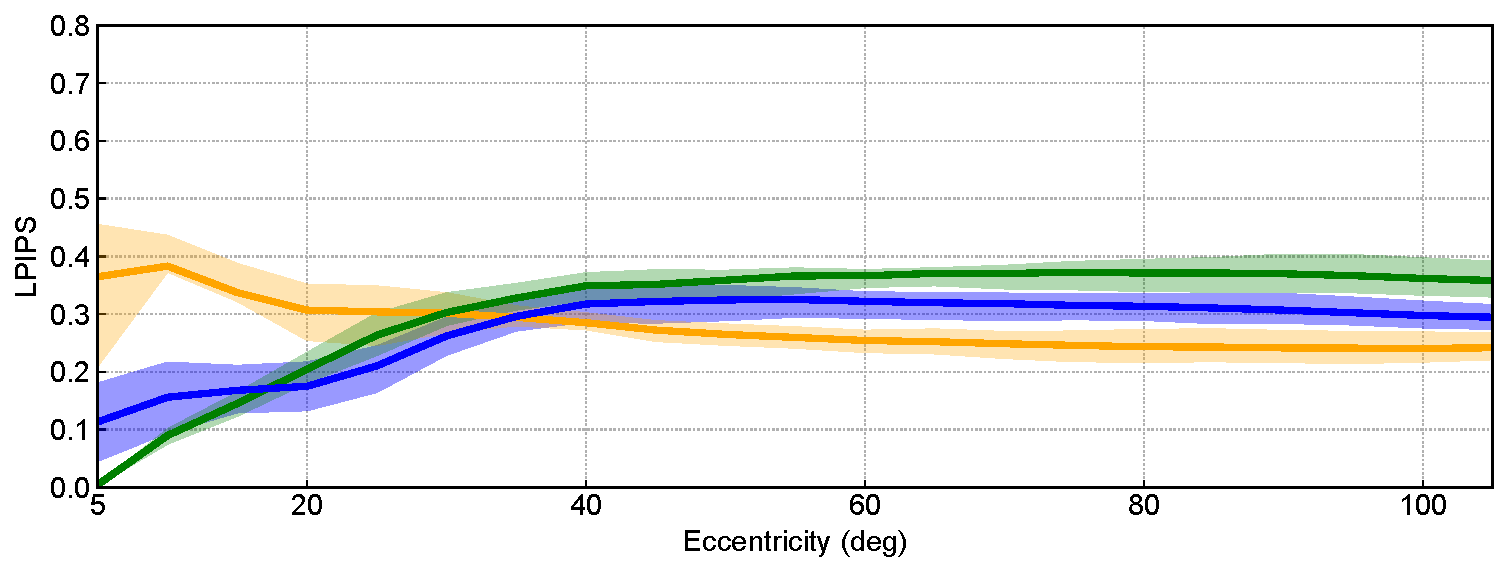
\includegraphics[width=0.48\linewidth]{TOG/figs/lpips_scenegas.pdf}}\label{fig:lpips:gas}
    \subfloat[minecraft]{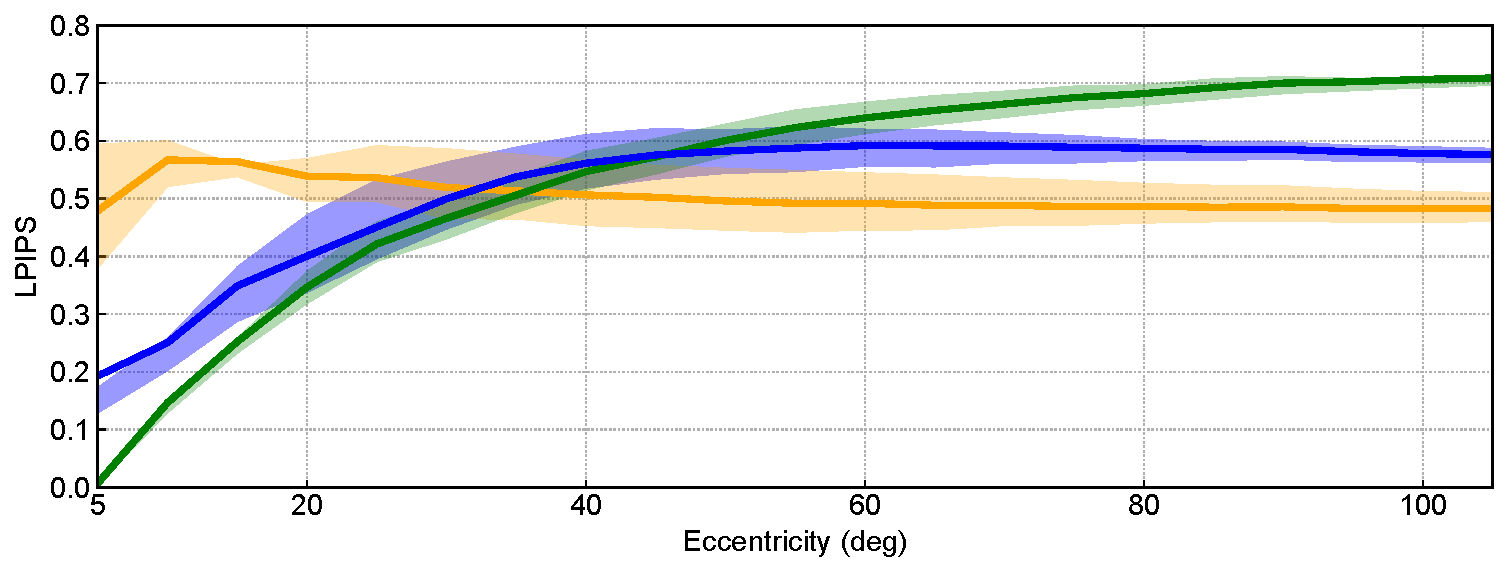
\includegraphics[width=0.48\linewidth]{TOG/figs/lpips_scenemc.pdf}}
    
    \subfloat[gallery]{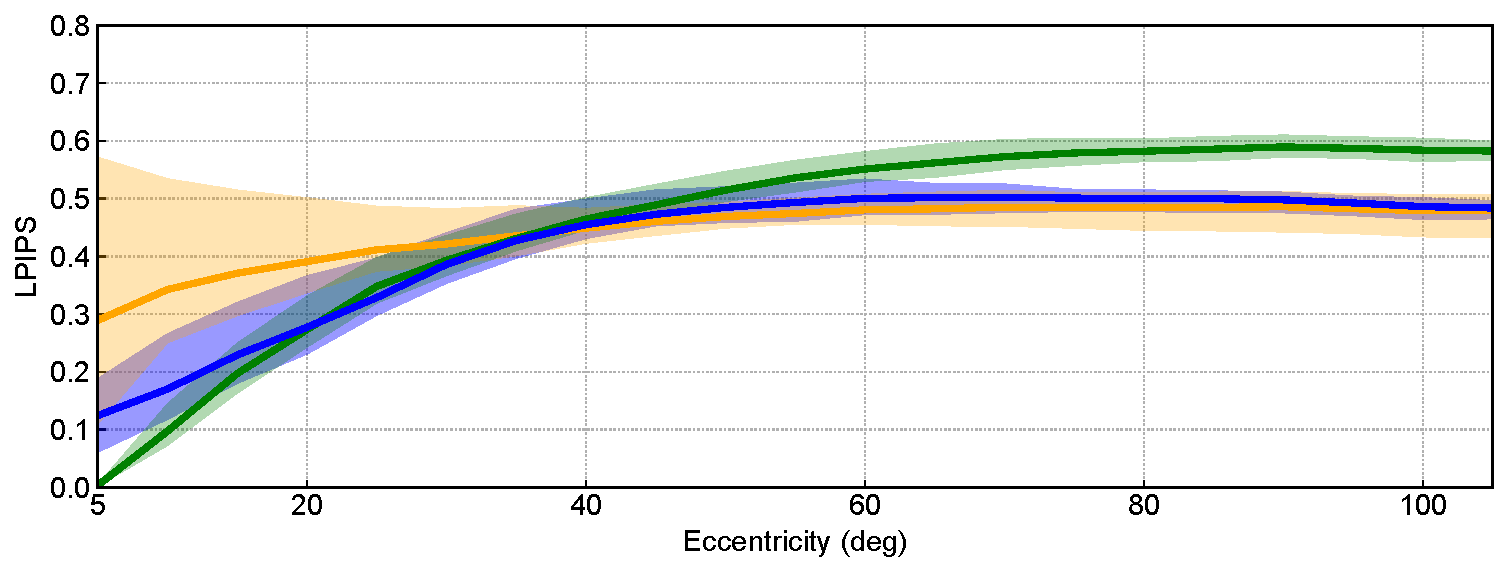
\includegraphics[width=0.48\linewidth]{TOG/figs/lpips_scenegallery.pdf}}
    \subfloat[bedroom]{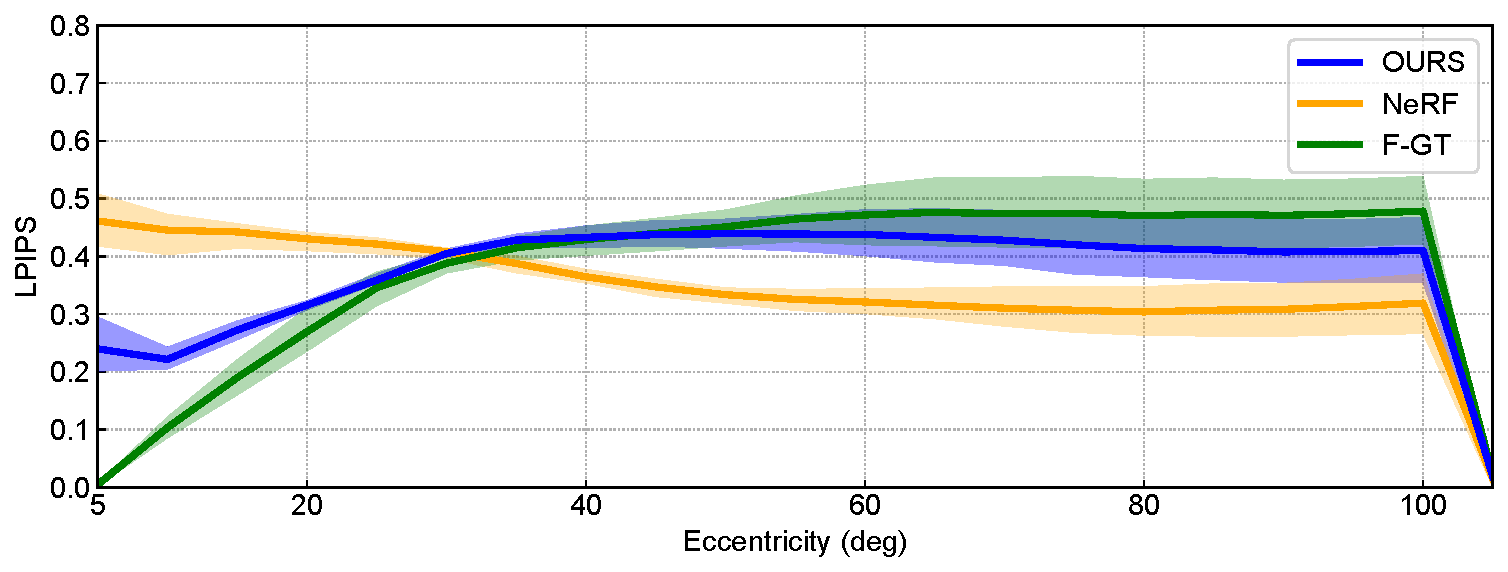
\includegraphics[width=0.48\linewidth]{TOG/figs/lpips_scenebedroom.pdf}}
    \caption{LPIPS analysis of all scenes as well as comparison of our method, NeRF, and foveated GT on each eccentricity.}
    {\zh{Add intersection lines later.}}
    \label{fig:lpips}
\end{figure*}

\subsection{Intra-System Workings}
\label{sec:study:intra}
\paragraph{Spatial-Temporal Optimality}

% apply objective metric to |cref{fig:optimization}, aka different sample numbers


\paragraph{Ablation Study}
% the performance of an AI system by removing certain components, to understand the contribution of the component to the overall system

% nmsl v.s. msl